In this Chapter we will present the results of implemented the previously specified requirements that originated the Socii tool. As we previously mentioned we
choose a set of requirements (among a big list of possibilities) that would allows us to have a tool with the most relevant and core functionalities
in order to prove our hypothesis of building a web based \glspl{sna} tool.\\
\indent Along the Chapter we will not only list results but show them as well, in some of the following sections we present a set of Socii images that depict the implemented functionalities and how to use them. In a more final part of this Chapter we present a case study, were we analyze a real network and derive some different conclusions that well demonstrate some of the use cases of Socii.

%% ---------------------------------------------- Note about the final results
\section{Note about the final results}

As the development of the tool depended on the \glspl{osn} integration and real data analysis, we had to somehow manage to fed real data sets into
Socii. The way we achieve this was not an totally automatic process, we used the crawler modules and extraction \glspl{api} mentioned and very well explained in Chapter 5 and 6, to extract real data sets into a local filesystem, and then with a migration script we pointed to the production MongoDB instance in order to store the real data so that Socii aggregator component could get the real data. To improve data feeding interoperability we have two functionalities working side by side, the user may choose to analyze a real network (previously extracted by the mentined process) or the user may choose to generate a network with data from our generators module.


%% ---------------------------------------------- Final Results Summarization
\section{Final Results Summarization}

The following table summarizes the features that were implemented on Socii. All the "\textbf{MUST}" requirements were implemented
and two additional "\textbf{SHOULD}" requirements were also implemented since they were almost cost free once we had the
component react-d3-graph in a more advanced stage. As mean of summarization we will present a table concisely points to
each requirement with the proper reference that we created in Chapter 6.

\begin{table}[H]
\renewcommand{\tabcolsep}{2pt}
\begin{tabular}{ |c|l|c| }
\hline
\textbf{Requirement} & \textbf{Short Description} & \textbf{Status}\\
\hline
6.3.2, 1 & Socci login & \ding{51}\\
\hline
6.3.2, 2 & Order network build (extraction simulation) & \ding{51}\\
\hline
6.3.2, 3 & Extraction feedback & \ding{51}\\
\hline
6.3.3, 1 & Render network & \ding{51}\\
\hline
6.3.3, 2 & Community detection (visually identifiable) & \ding{51}\\
\hline
6.3.3, 3 & Drag and Drop all network & \ding{51}\\
\hline
6.3.3, 4 & Zooming interactions & \ding{51}\\
\hline
6.3.3, 5 & Interactive node comparison & \ding{51}\\
\hline
6.3.3, 6 \begin{small}(should requirement)\end{small} & Global network interactions (Toolbar) & \ding{51}\\
\hline
6.3.3, 7 \begin{small}(should requirement)\end{small} & Disable heavy animations & \ding{51}\\
\hline
6.3.2, 1 & Network Generator (Facebook) & \ding{51}\\
\hline
6.3.2, 1 & Network Generator (LinkedIn) & \ding{51}\\
\hline
6.3.2, 2 & Network Generator - Configuration & \ding{51}\\
\hline
6.3.3, 4 & Zoom network & \ding{51}\\
\hline
6.3.3, 5 & Detect heavy network and disable animations & \ding{51}\\
\hline
6.3.4, 1 & Render label along side each node & \ding{51}\\
\hline
6.3.4, 2 & Highlight node and adjacent connections & \ding{51}\\
\hline
6.3.4, 3 & \begin{tabular}{@{}l@{}}Node click and show information\\ (network metrics and information in\\ the context of the \glspl{osn})\end{tabular} & \ding{51}\\
\hline
6.3.4, 4 & Drag and Drop nodes & \ding{51}\\
\hline
6.3.5, 1 & Render network links with \textit{semantic thickness} & \ding{51}\\
\hline
6.3.8, 1 & Download network in the format GraphML & \ding{51}\\
\hline
\end{tabular}
\caption{\label{table:featuresocii} Summarization of Socii features.}
\end{table}

In the Table \ref{table:featuresocii} we present a list of the implemented requirements, these refer to the requirements in Chapter 6. All the requirements are \textbf{MUST} requirements unless otherwise is stated.


%% ---------------------------------------------- Socii - final aspect and functionalities
\section{Socii - final aspect and functionalities}
In this section we do an overview across Socci application, we present the overall functionalities that Socii offers
from an end user perspective.

\subsection{Network Configuration Area}

\subsubsection*{Entry state}

\begin{figure}[h!]
\begin{center}
  \hspace*{-0.8in}
  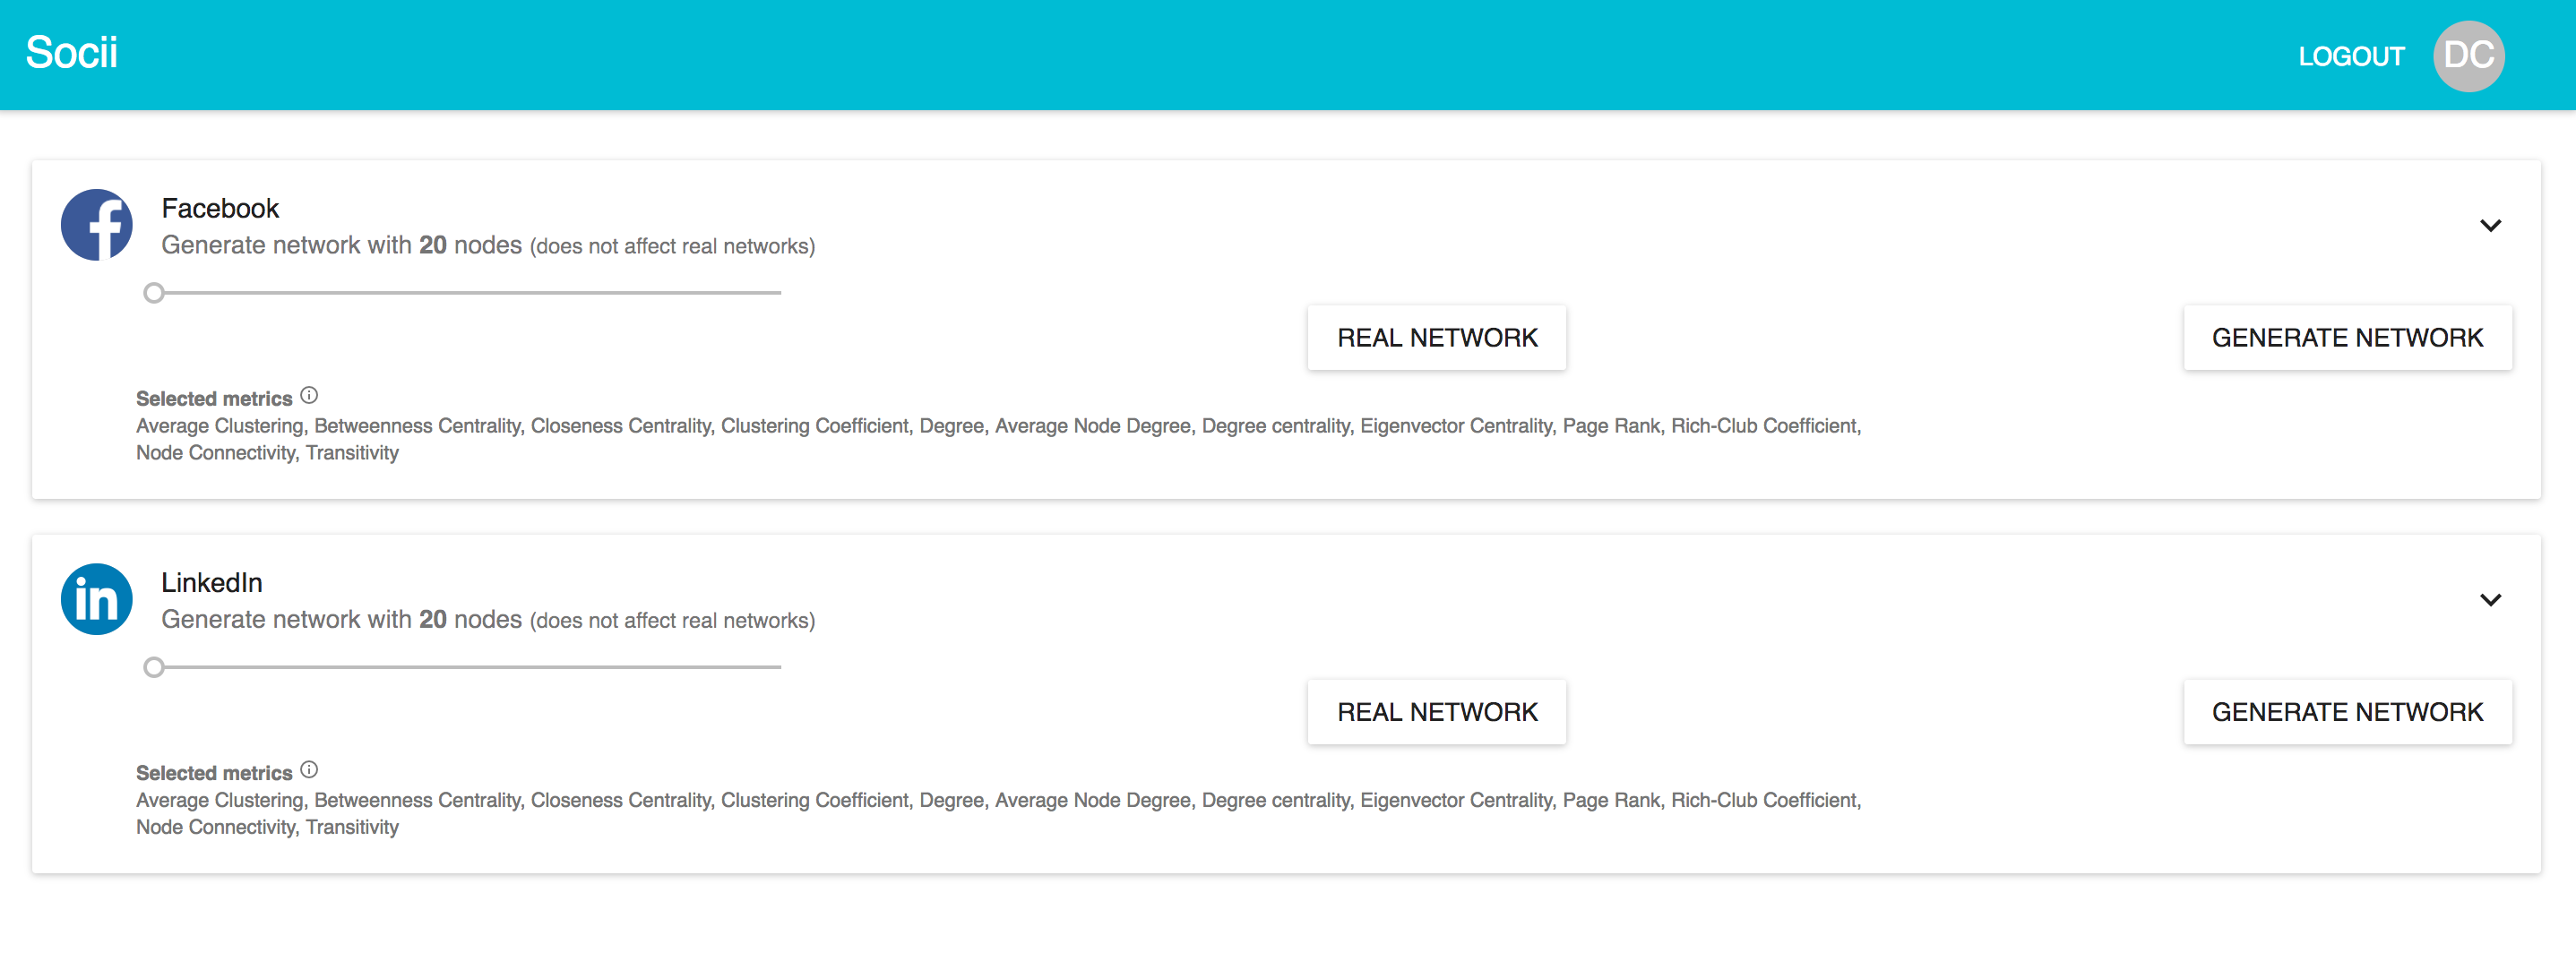
\includegraphics[width=1.2\textwidth]{img/socii/socii_1.png}
\end{center}
\caption{\label{img:socii_1} Socii landing page. Network configuration area.}
\end{figure}

In Figure \ref{img:socii_1} we may observe our initial page where we display available \glspl{osn} that can be configured in this area and then a network generation or network calculation upon real network may be ordered. Each \glspl{osn} consists in a expandable card that once expanded contains all the details and information about the \glspl{osn} and metrics configuration.

\subsubsection*{Configuration card detail}

\begin{figure}[h!]
\begin{center}
  \hspace*{-0.8in}
  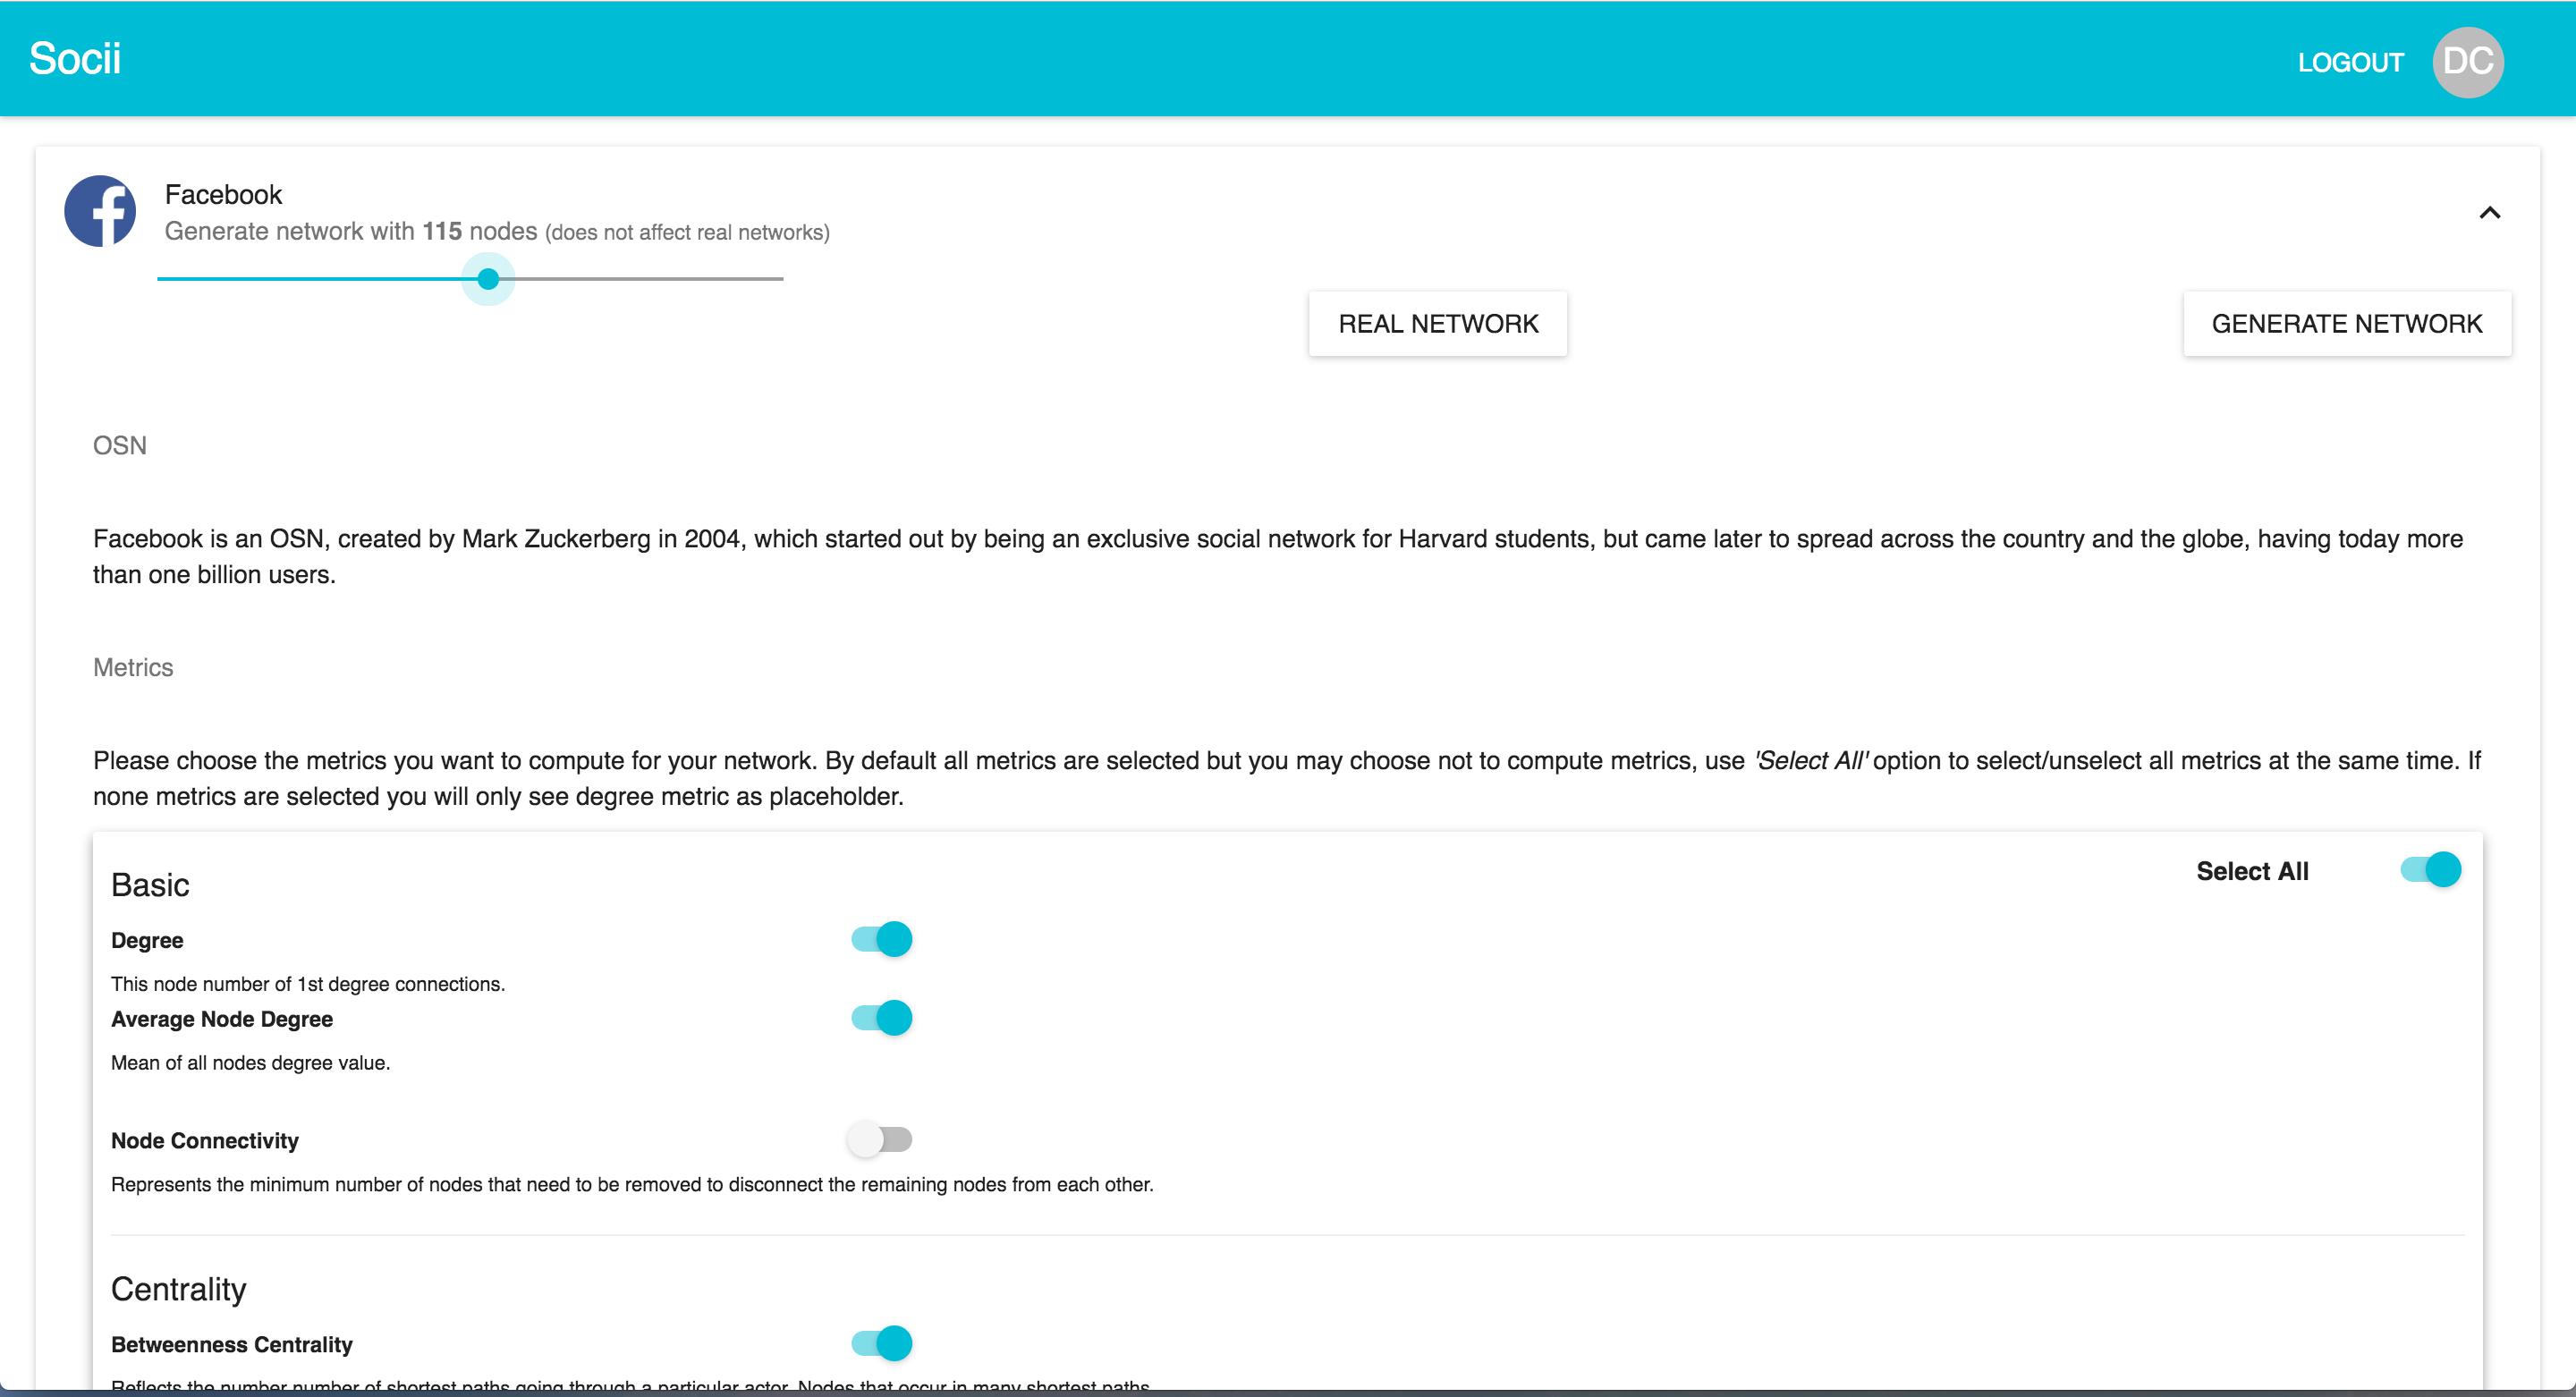
\includegraphics[width=1.2\textwidth]{img/socii/socii_2.png}
\end{center}
\caption{\label{img:socii_2} Network configuration area. Facebook configuration expanded.}
\end{figure}

In Figure \ref{img:socii_2} Facebook configuration card is expanded and here we see that we can have a great level of granularity upon the \glspl{sna} metrics that we want to calculate against a certain network. On the top of the card we have a brief description of the \gls{osn} followed by sections that represents sets of metrics, and for each one of the metrics we also provide a brief explanation for a given metric.\\
\indent These are the metrics that we will then be able to see for each node in the network visualization area. To reach more flexibility we decide on switches visual elements to turn on/off a certain metric, by doing this we may combine any set or subset of metrics. Some of the metrics are global (these mean that they are calculated regarding the graph/network in general) other are node specific (have a meaning at node level), this is implicit within each metric description.

\subsection{Network Visualization Area}

\begin{figure}[h!]
\begin{center}
  \hspace*{-0.8in}
  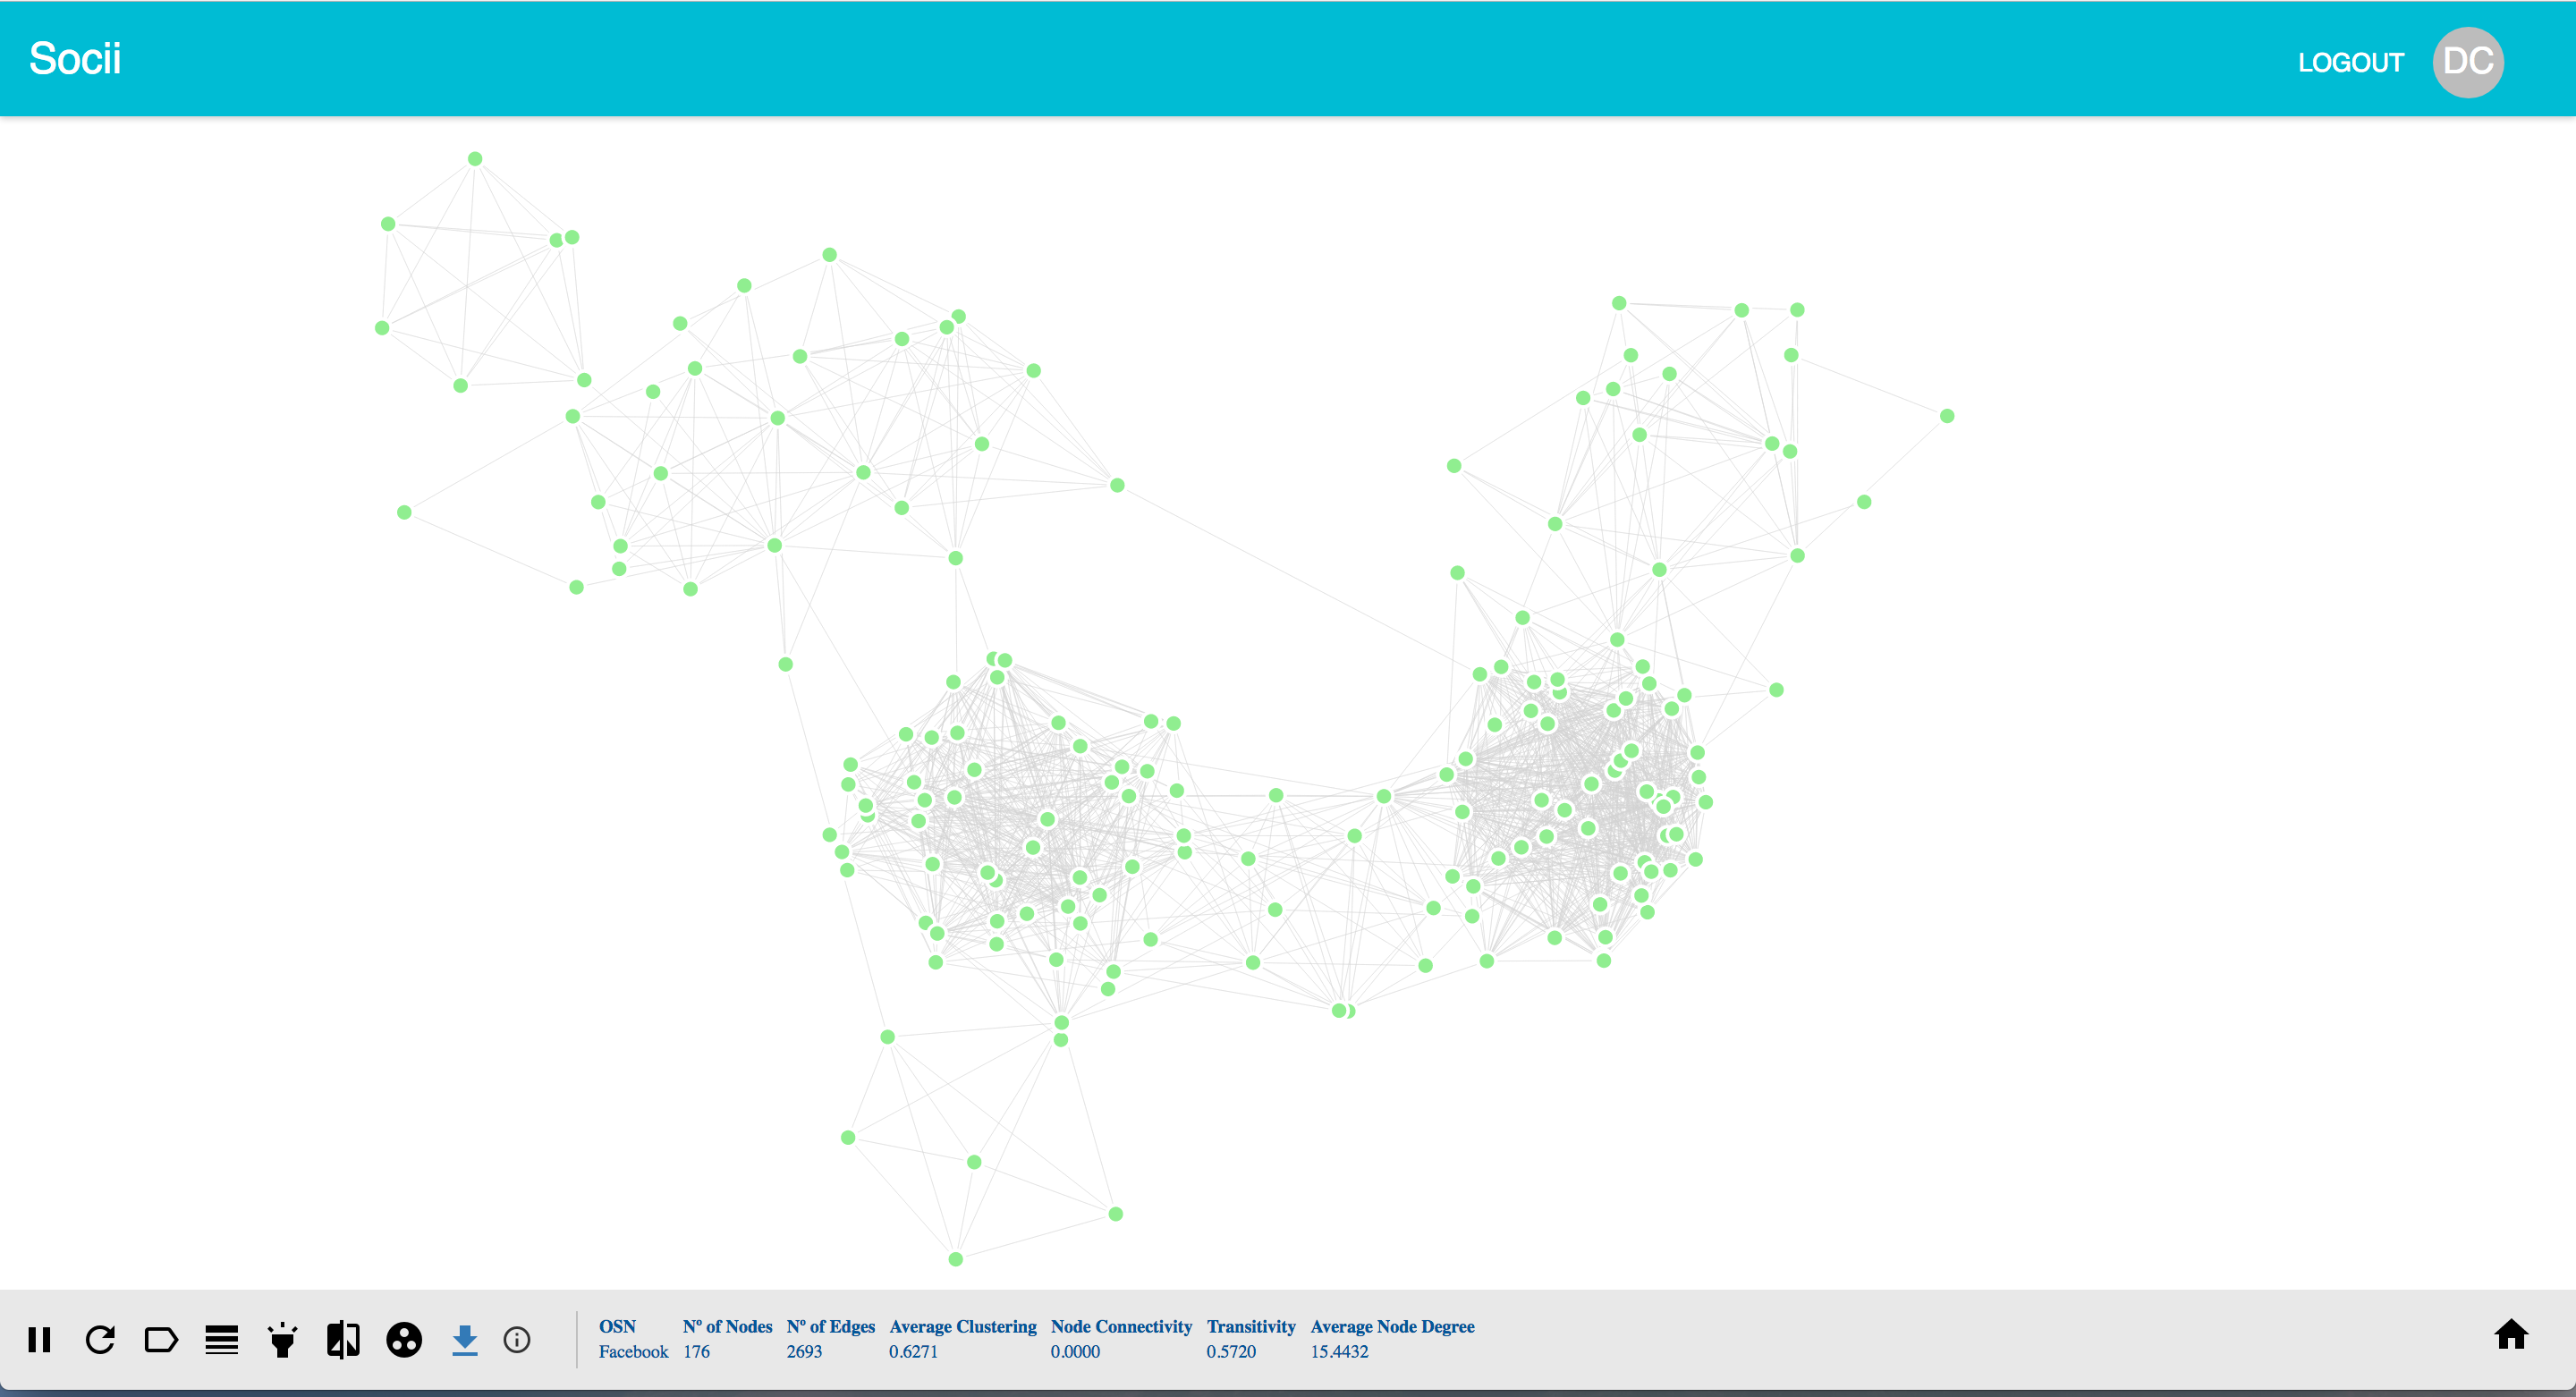
\includegraphics[width=1.2\textwidth]{img/socii/socii_3.png}
\end{center}
\caption{\label{img:socii_3} Network visualization area.}
\end{figure}

The network visualization are is the main area of Socii tool, here is where the user will actually be able to visualize and analyze a given social structure for a certain \gls{osn}. As we may observe in Figure \ref{img:socii_3}, we still have the app header where the user can logout at any time, below we have a large area where the network is rendered. At the bottom of the page we have the toolbar that contain among others, that will be explain latter with greater detail, main graph interactions such as pause animations or show/hide nodes labels.

\subsubsection{Toolbar}

\begin{figure}[h!]
\begin{center}
  \hspace*{-0.8in}
  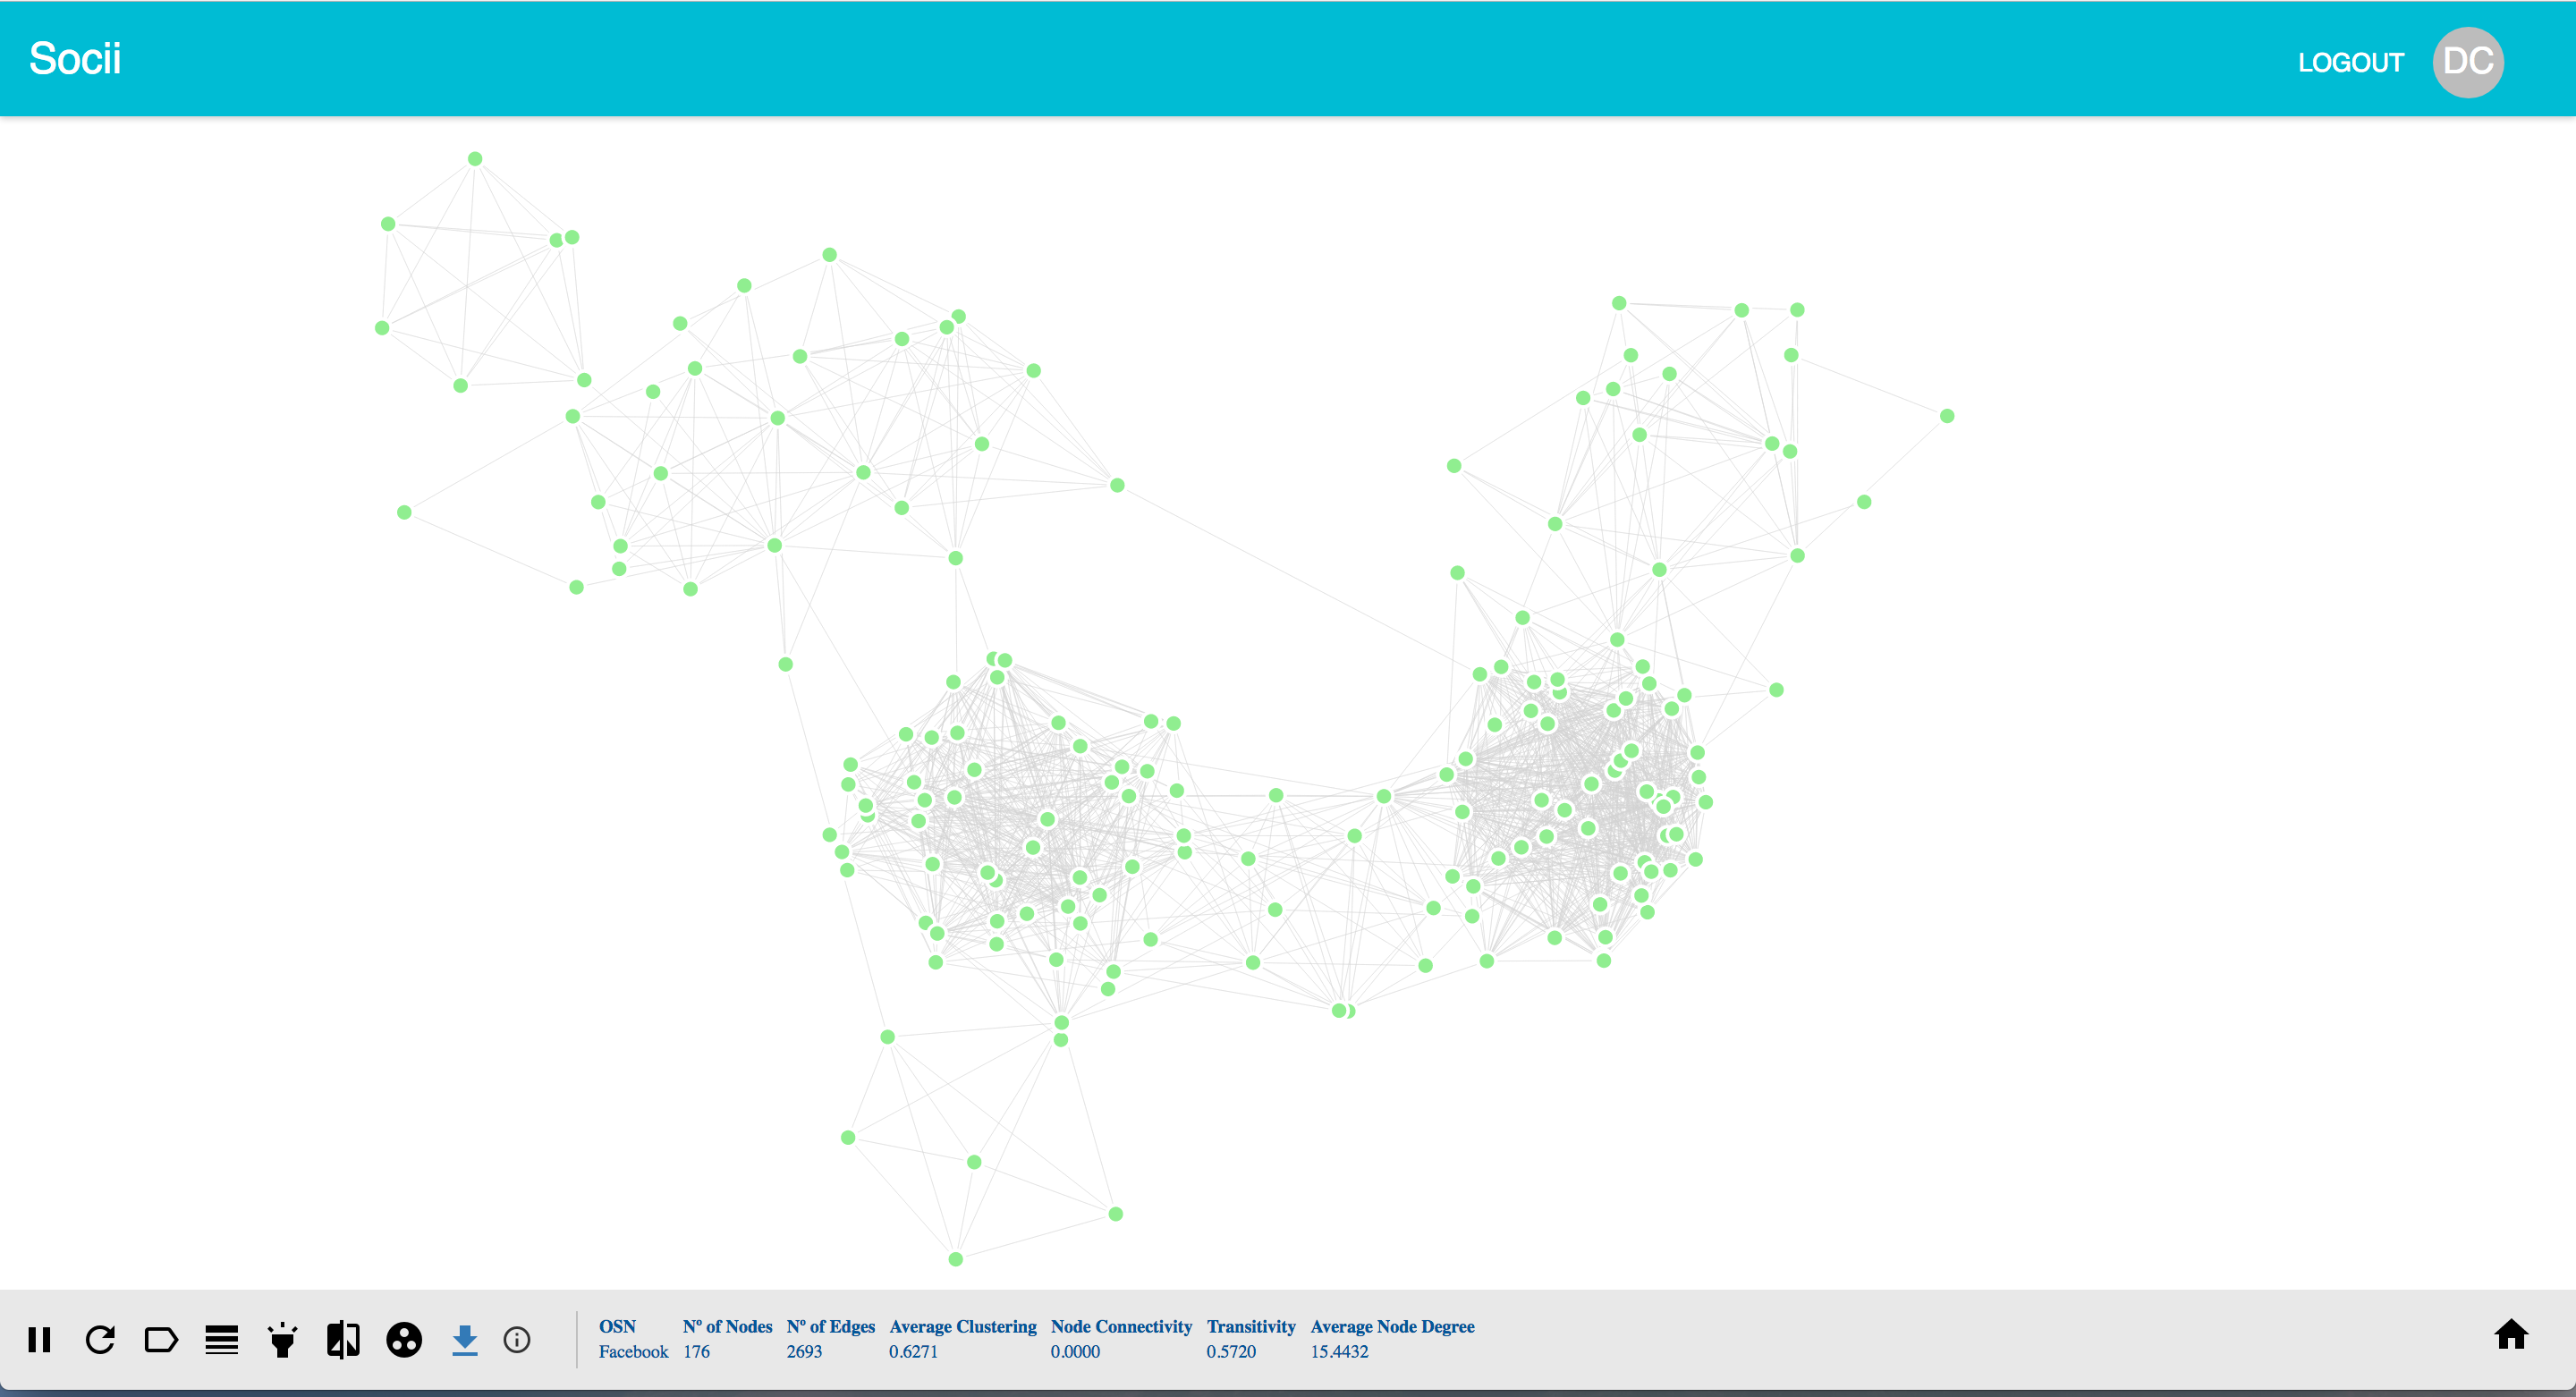
\includegraphics[width=1.2\textwidth]{img/socii/socii_3.png}
\end{center}
\caption{\label{img:socii_4} Dialog containing toolbar help information. At the bottom the toolbar.}
\end{figure}

In this particular section we will only focus on the toolbar and on the functionality that this application component offers. As we can see in image \ref{img:socii_4} we may observe an explanation of each icon present on the toolbar, this pop up descriptive dialog appears when the information icon (last icon counting from the left) is pressed, this will allow us to keep the toolbar clean (not having to render descriptions or labels at the side of the symbols) having only the toolbar with the icons and no additional descriptive content.\\
\indent Next we present the detailed description of each action/icon (icons are enumerated from left to right as displayed in the toolbar).
\begin{itemize}
    \item \textbf{pause} - the pause icon allows users to stop ongoing animations, this animations happened mainly at the start of the visualization when the network is still being arranged and nodes are being positioned to not overlap (this job is done by D3.js);
    \item \textbf{refresh/redo} - clicking this icon will make all the dragged nodes go back to their initial positions (approximately);
    \item \textbf{label/etiquette} - clicking in this icon shows and hides the labels of the nodes in the network, the user may use this as he pleases according to its visualization needs;
    \item \textbf{strokes} - clicking this icon will make nodes connections semantic visually, this means that the link thickness will be propositional to the number of common relations between the two parts;
    \item \textbf{LANTERNA} - when this feature is active the user is able to mouse over nodes in the network and to stand out the selected nodes relations (only the mouse hovered node relationships 1st and 2nd degree will be highlighted);
    \item \textbf{switch/compare} - activating this feature will make the clicked nodes comparable. This means that when we click on some 1st and then a 2nd node, we will be able to compare this two nodes at the most granular level (this feature is explained in the Node Comparison section);
    \item \textbf{circle/community} - clicking here opens a pop up dialog form that allows users to perform some community detection studies on the network, this is explained in the Community Detection section;
    \item \textbf{arrow/download} - when the user clicks the downloaded icon a GraphML file is generated and download containing the rendered network basic structure.
\end{itemize}

\indent After this actions/icons section the toolbar presents some global metadata about the rendered network. This information consists in: the \gls{osn} name, the number of rendered nodes and links and some global metrics such as average clustering coefficient and average node degree.

\subsubsection{Node Discovery}

\begin{figure}[h!]
\begin{center}
  \hspace*{-0.8in}
  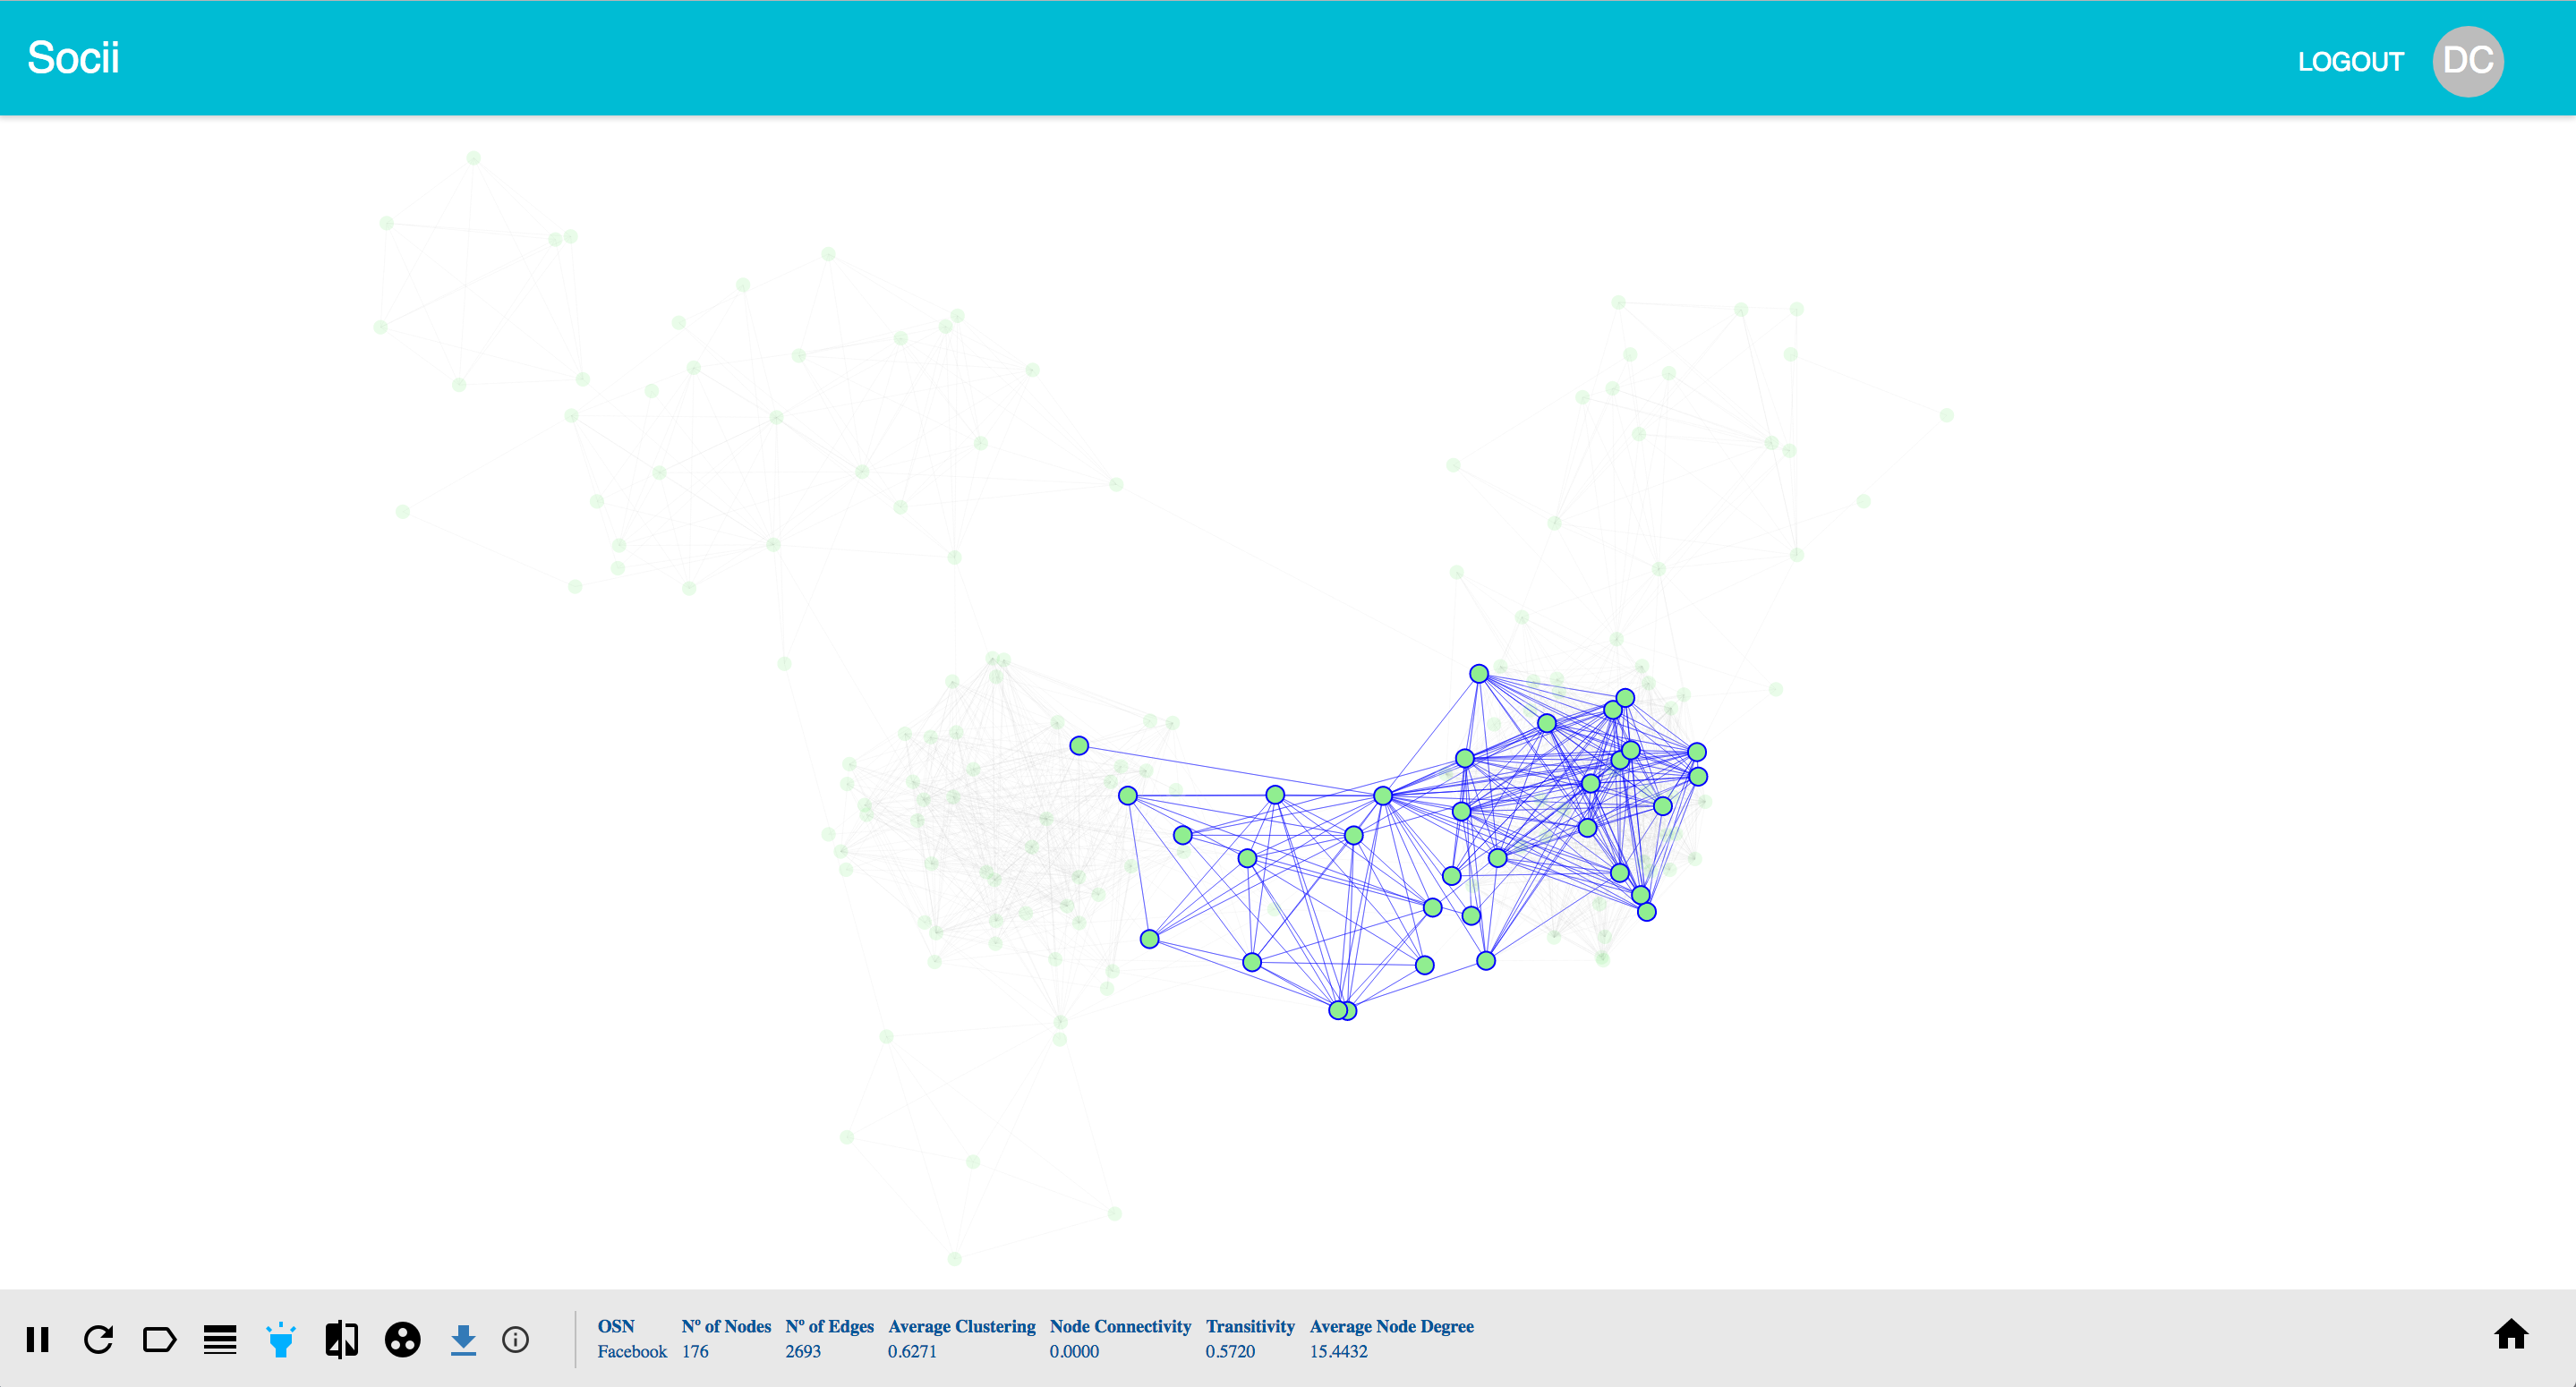
\includegraphics[width=1.2\textwidth]{img/socii/socii_5.png}
\end{center}
\caption{\label{img:socii_5} Node discovery feature.}
\end{figure}

Node discover allows us to stand out some nodes upon the rest of the network. When we mouse over some node we will highlight that nodes and its 1st and 2nd degree connections, as we can see in the example provided in the Figure \ref{img:socii_5}

\subsubsection{Node Details}

\begin{figure}[h!]
\begin{center}
  \hspace*{-0.8in}
  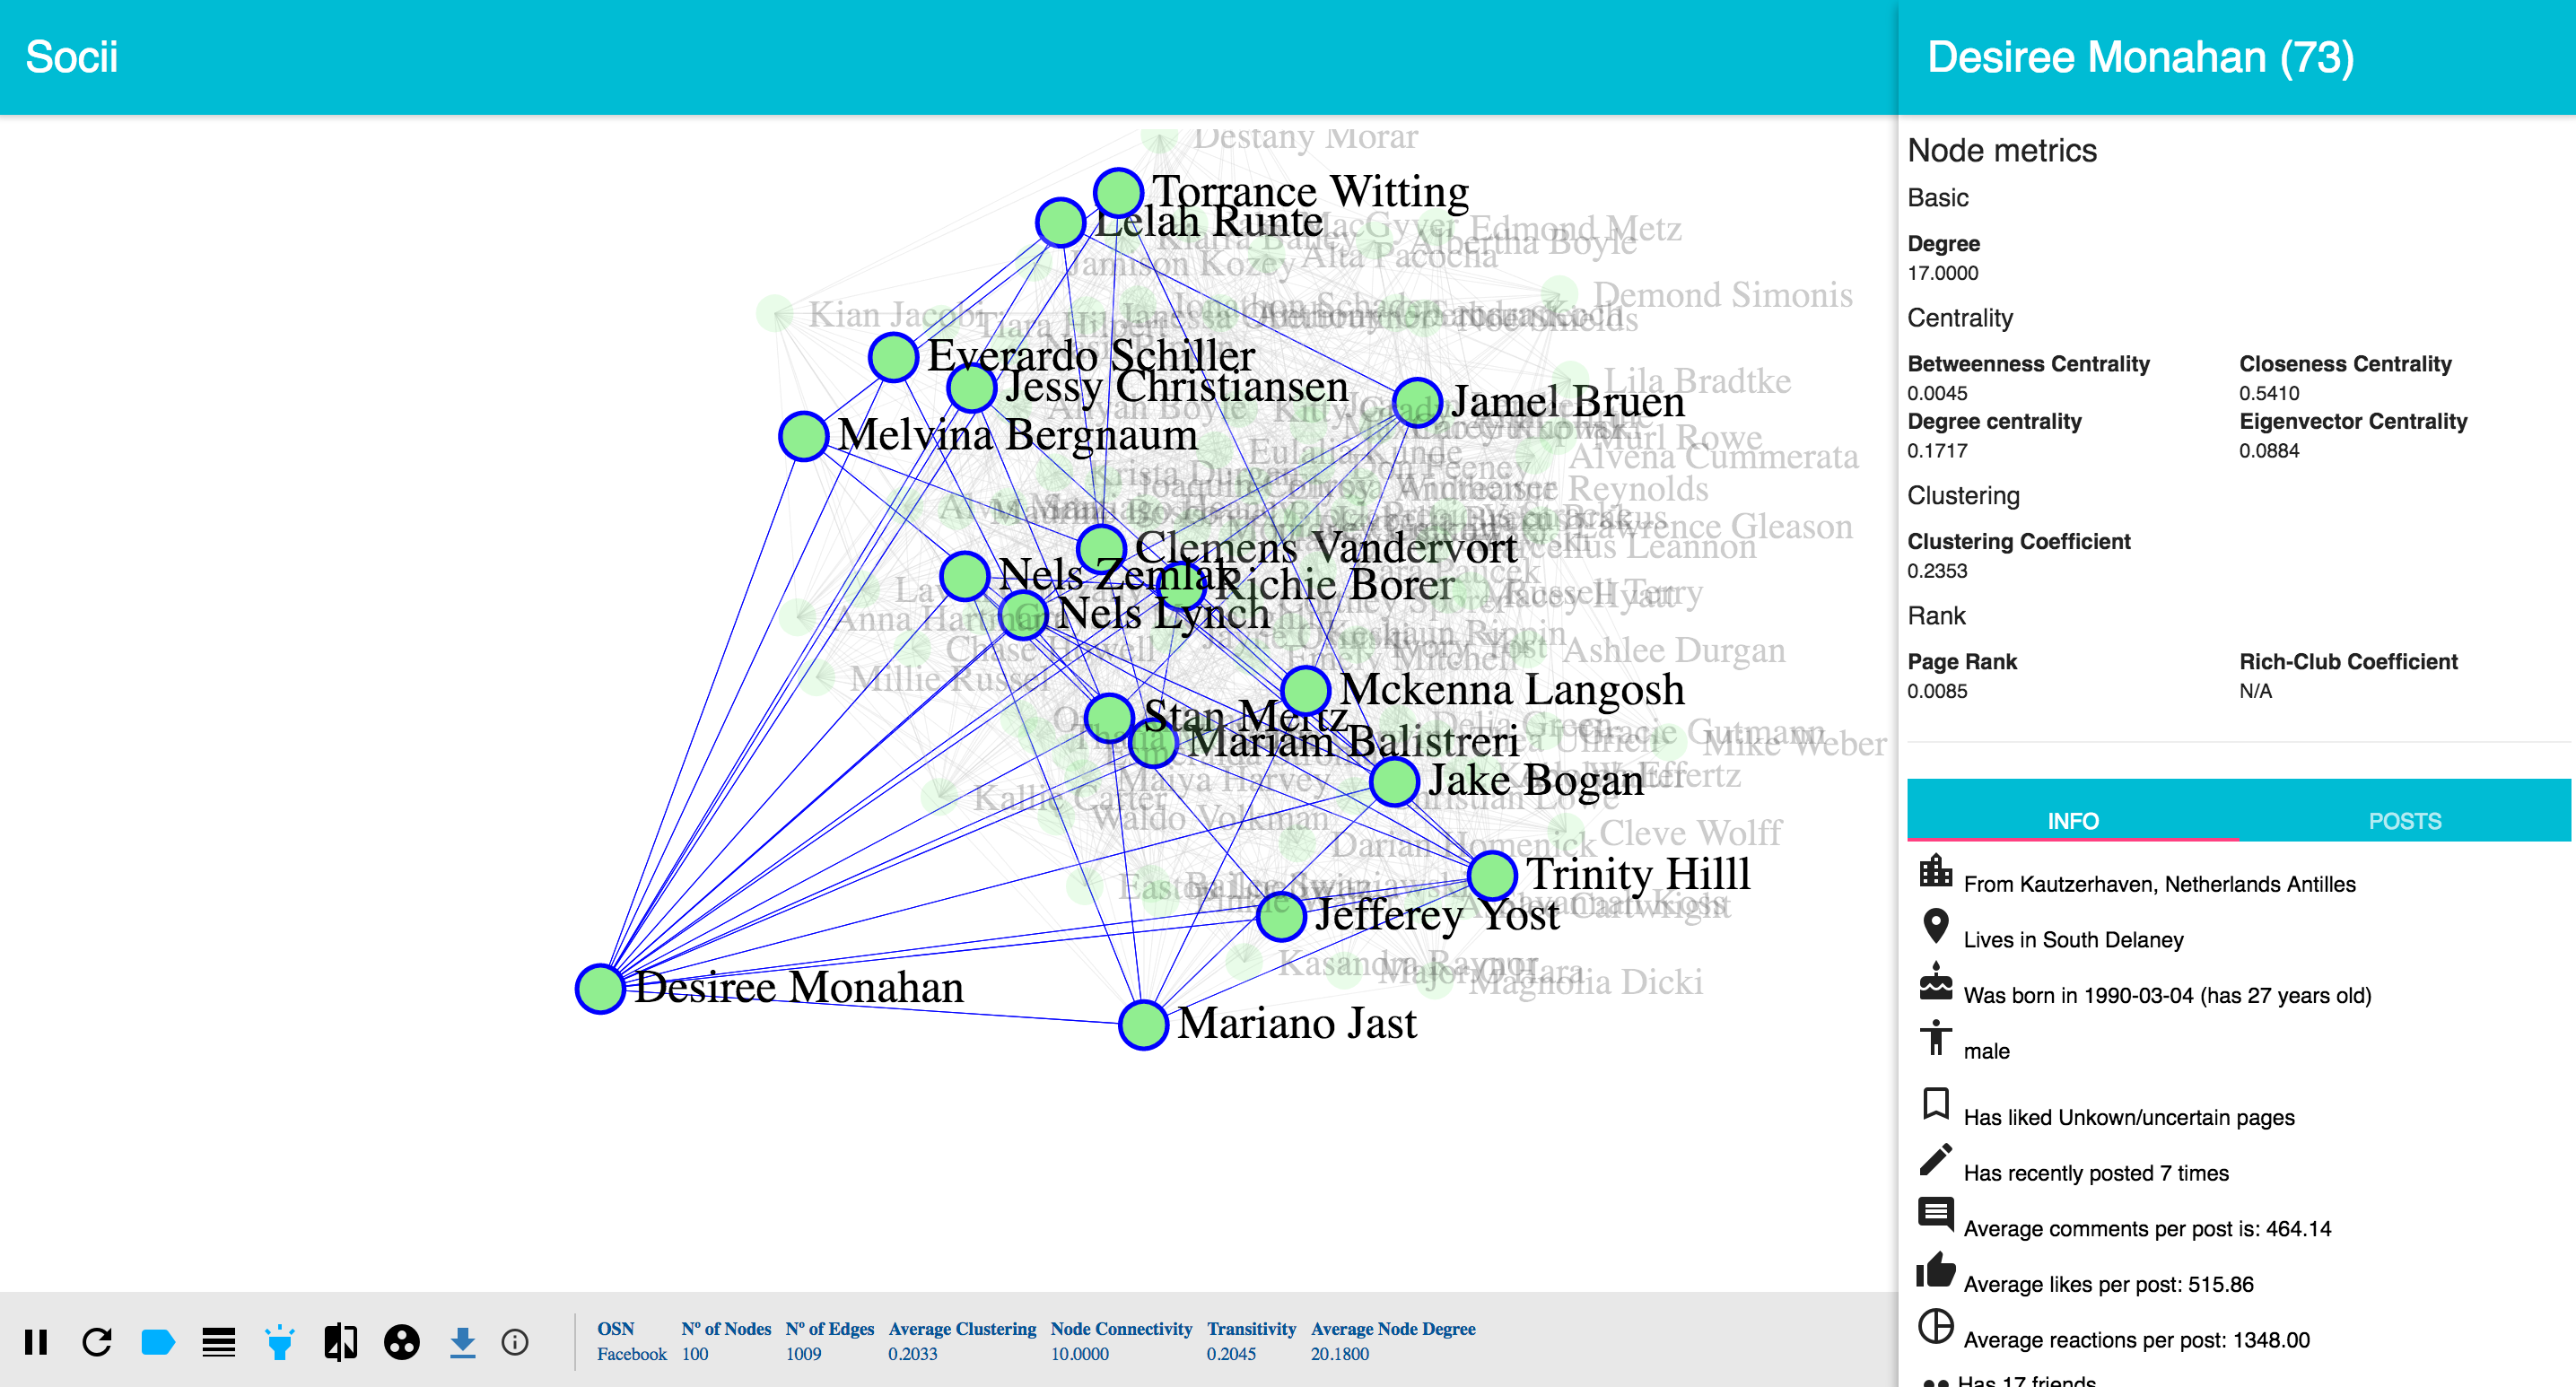
\includegraphics[width=1.2\textwidth]{img/socii/socii_6.png}
\end{center}
\caption{\label{img:socii_6} Node details panel opens on the right side of the screen.}
\end{figure}

When clicking on some network node a right side panel will slide and display all that node information, this information includes the computed \gls{sna} requested metrics and the \gls{osn} data that appears in a more fashionable way.

\subsubsection{Node Comparison}

\begin{figure}[h!]
\begin{center}
  \hspace*{-0.8in}
  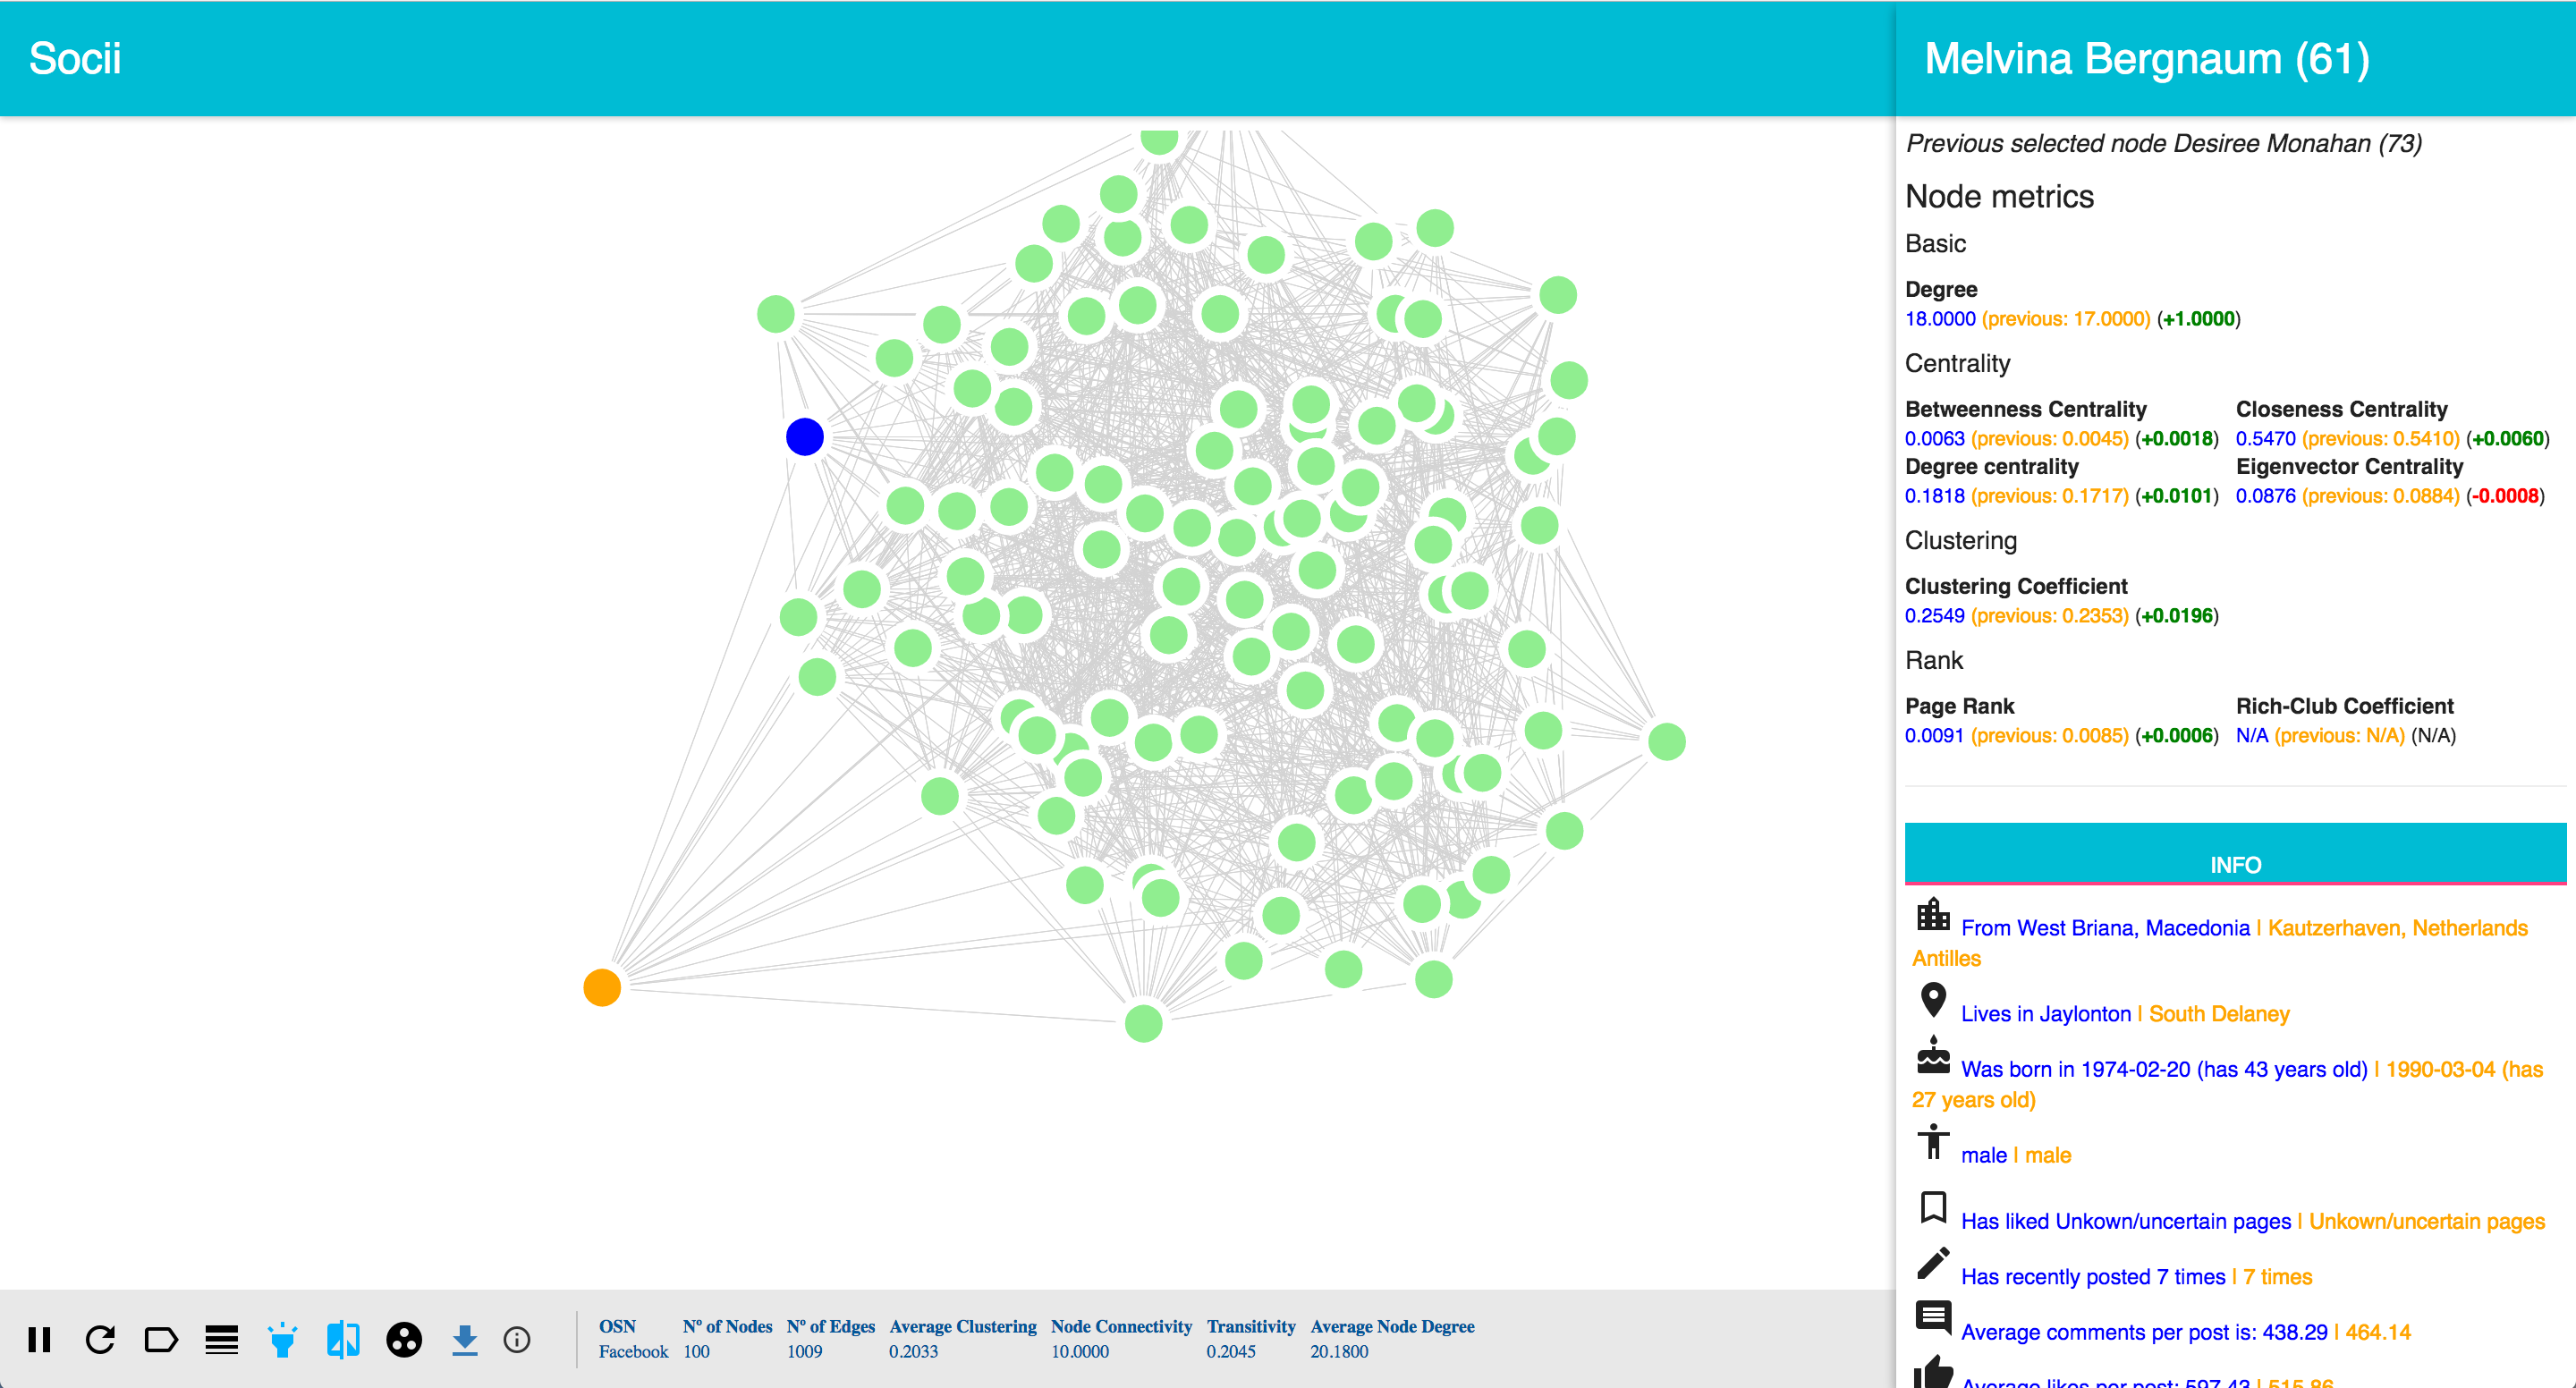
\includegraphics[width=1.2\textwidth]{img/socii/socii_7.png}
\end{center}
\caption{\label{img:socii_7} In the right side panel we may observe the detail of the selected nodes.}
\end{figure}

When activating node comparison functionality the user is able to compare two distinct nodes anywhere in the network (this said, they don't need to be connected so that we are able to compare them). But in what really consists this node comparison? It simply allows us to visualize in a comprehensive manner the metrics and \gls{osn} data of each one of the nodes simultaneously so that we don't have to jump between some two nodes details in order to compare them.\\
\indent As we can observe in Figure \ref{img:socii_7}, we can simultaneously see the metrics of the \textcolor{blue}{blue} (that represents the last node that the user clicked), and the the \textcolor{orange}{orange} node (color that represents the previous selected node).

\subsubsection{Community Detection}

This feature is one of the most crucial because it allows us to intercept individuals properties/attributes and intercept them at a large scale.\\
\indent Community detection functionlaity allows users to coloring the network according to some individuals \gls{osn} specific data property such as \textit{where the users live} or \textbf{what the are the users gender}, allowing us to perceive community patterns and identify communities based on a certain PRESSUPOSTO. Also we may made available a special property that allows users to be colored in terms of what Facebook pages they have liked.

\subsubsection*{Community by user properties}

\begin{figure}[h!]
\begin{center}
  \hspace*{-0.8in}
  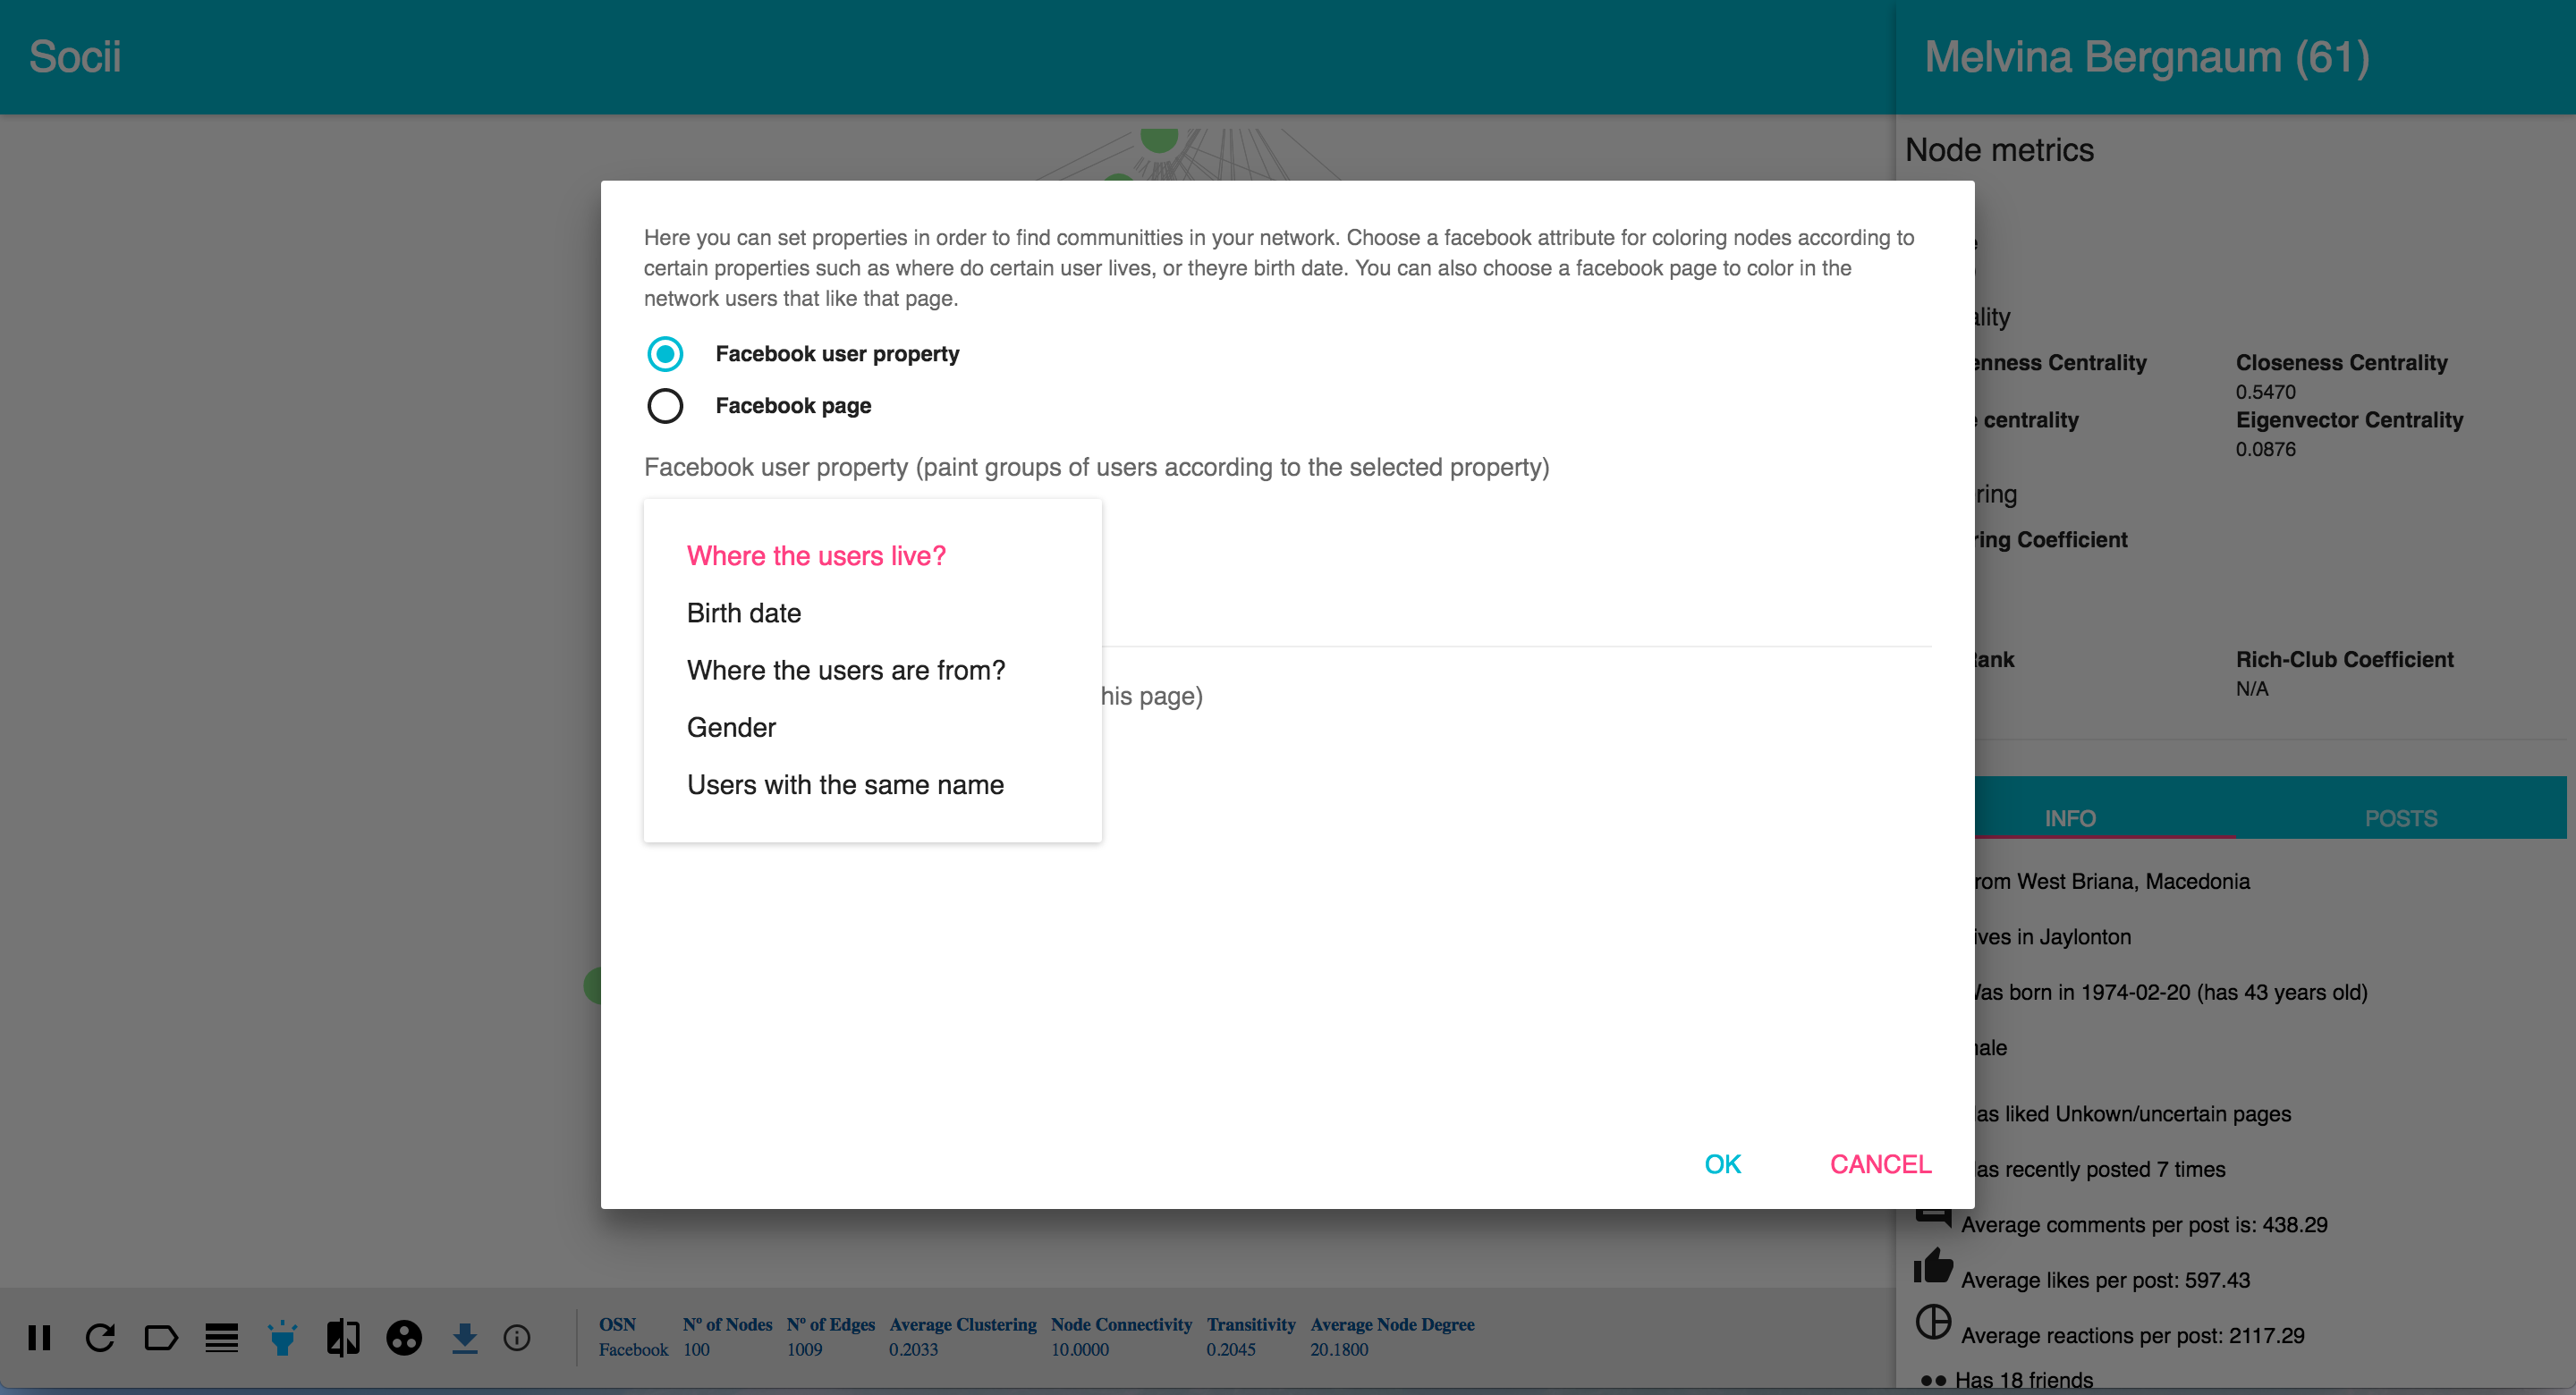
\includegraphics[width=1.2\textwidth]{img/socii/socii_8.png}
\end{center}
\caption{\label{img:socii_8} Pop up where user can configure community detection settings.}
\end{figure}

In Figure \ref{img:socii_8} we may observe how the user may choose to color the network by simply choosing a \textbf{"key question"}. The questions available what the result that they produce are the follwing:

\begin{itemize}
    \item \textbf{Where the users live?} - by choosing this option the all the users that have a common residence (current address) will be colored with the same color \footnote{\textbf{Note for future reference}: our color generator mechanism makes sure that no color collision happens, still, some colors may be the same with different tonalities};
    \item \textbf{Birth date?} - individuals with the same birth date will have the same color;
    \item \textbf{Where the users are from?} - individuals with the same place of birth will have the same color;
    \item \textbf{Gender} - individuals with the same gender will have the same color;
    \item \textbf{Users with the same name?} - users with the same name will have the same color.
\end{itemize}

\begin{figure}[h!]
\begin{center}
  \hspace*{-0.8in}
  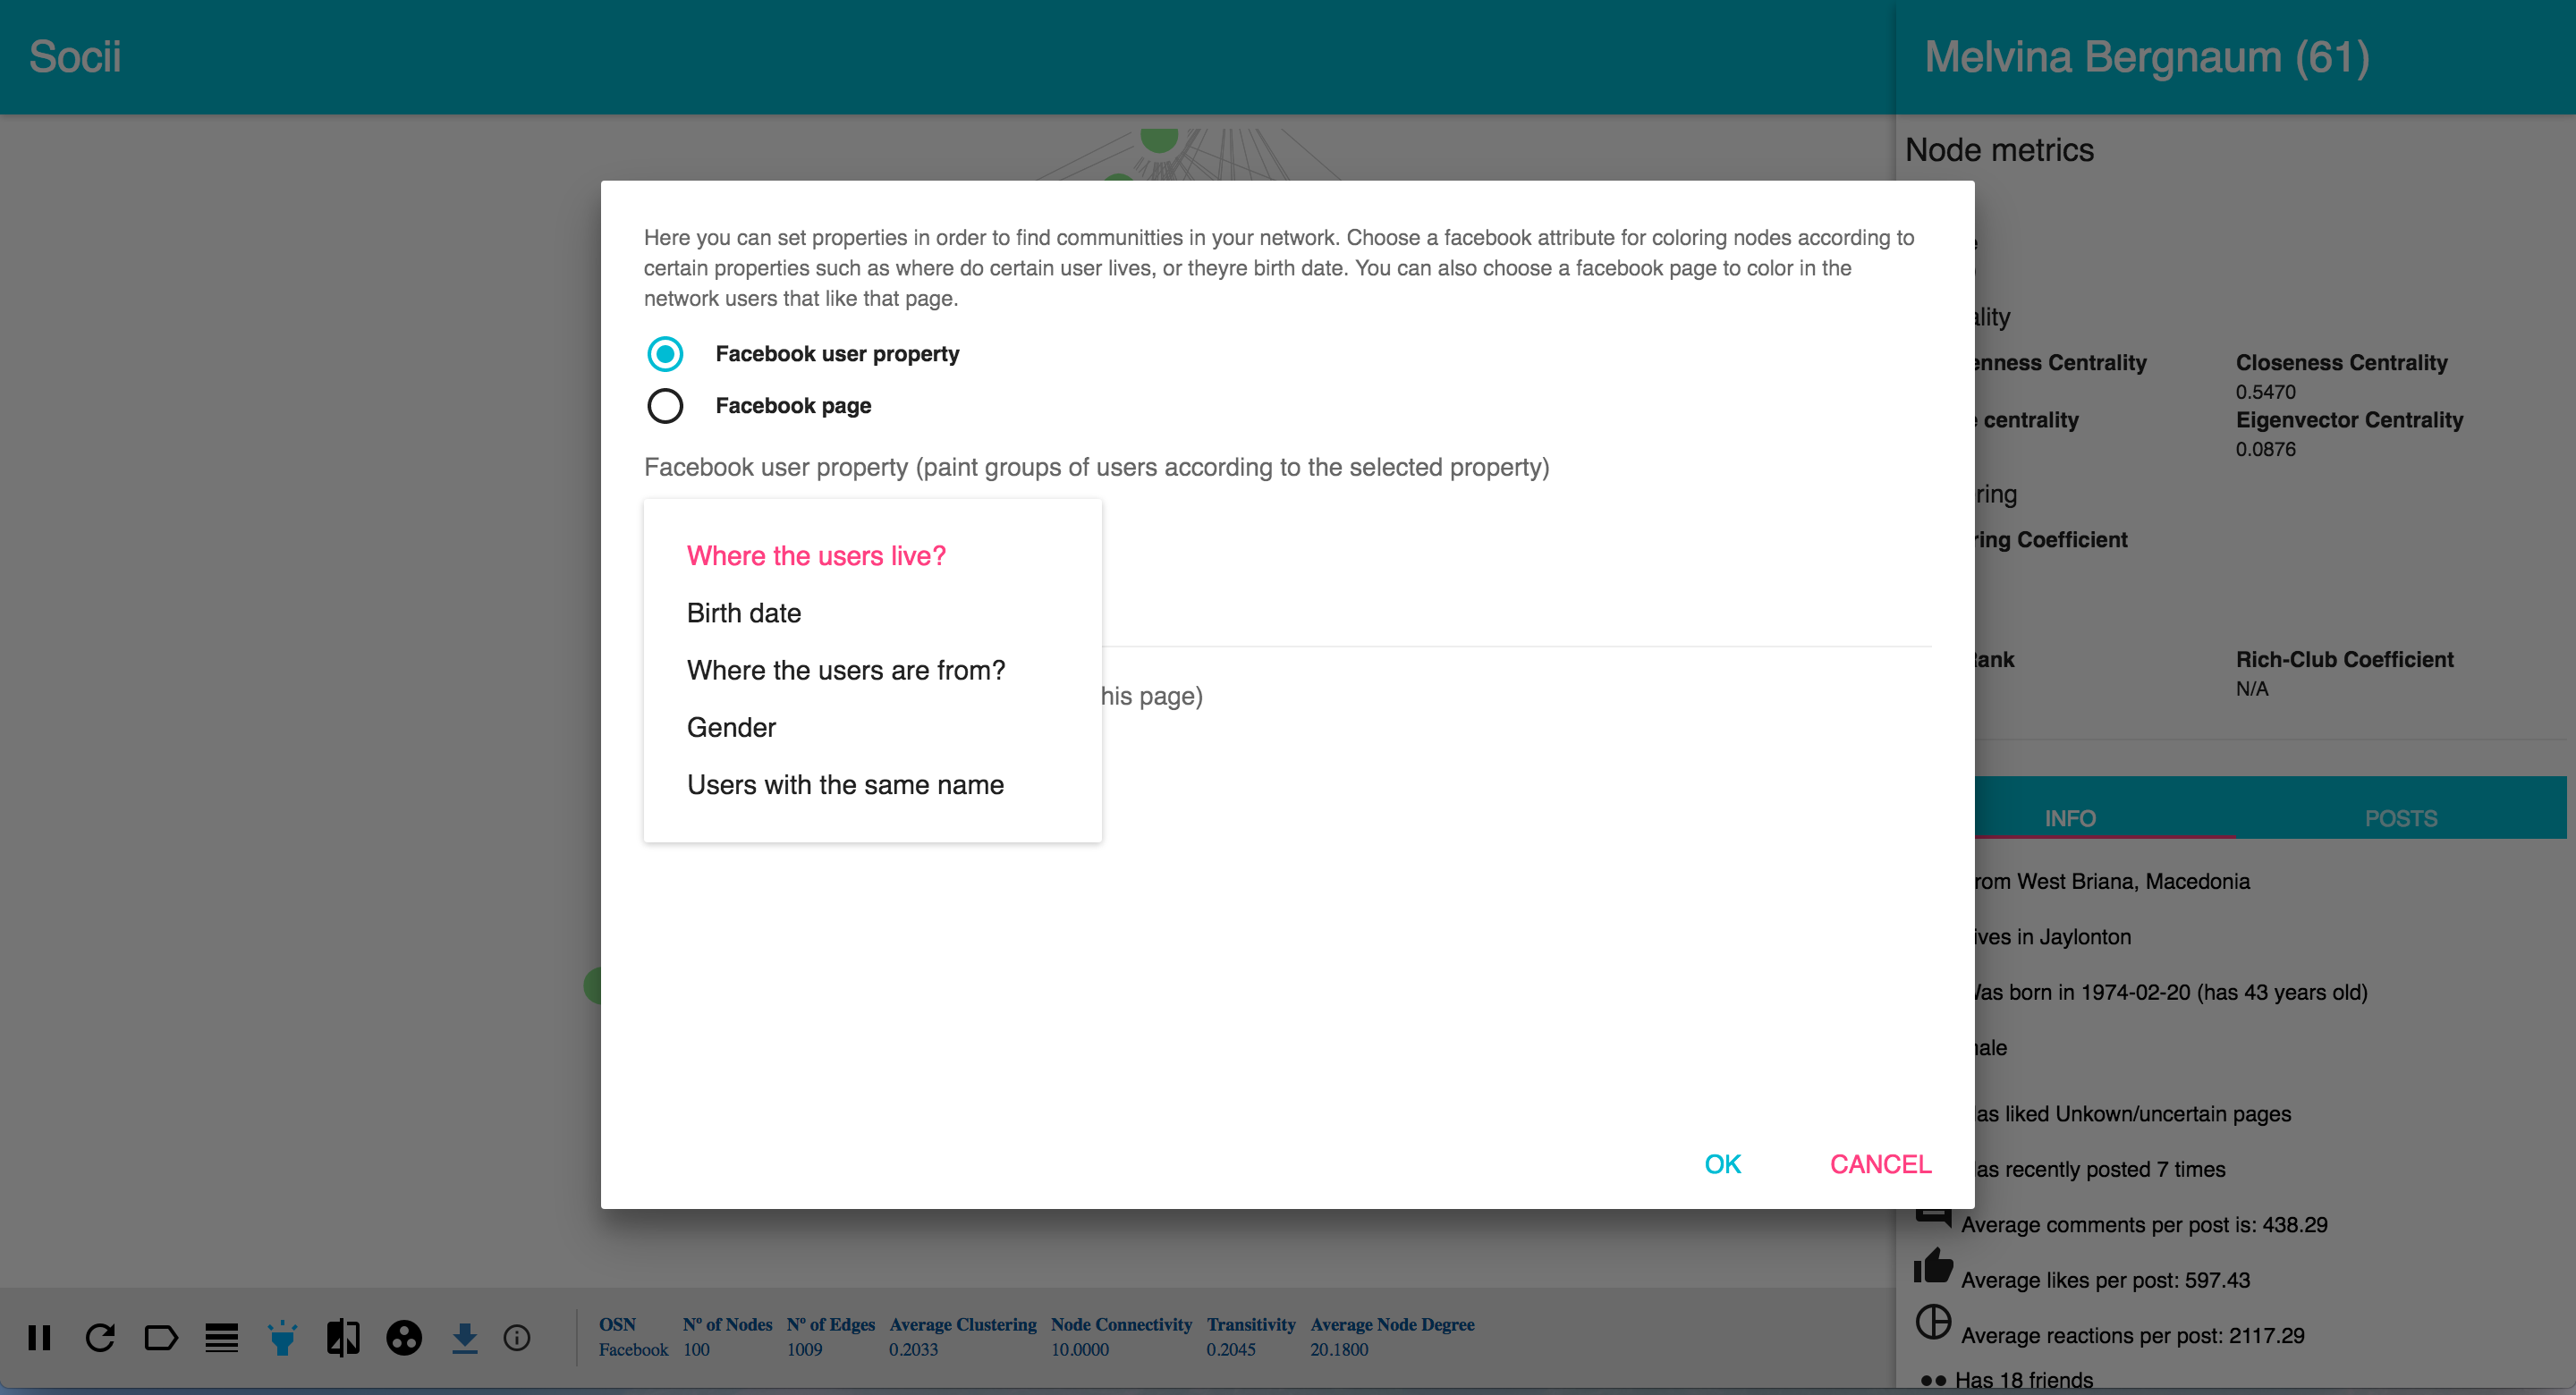
\includegraphics[width=1.2\textwidth]{img/socii/socii_8.png}
\end{center}
\caption{\label{img:socii_9} Community detection: \textbf{"Where the user lives?"}.}
\end{figure}

In Figure \ref{img:socii_9} we may observe the result of having detected individuals with the same place of birth.

\subsubsection*{Community by Facebook page likes}

By coloring individuals by a specific Facebook page like we can track users preferences within the network, this preferences can be anything (sports, Hollywood stars, food, shoes brand, tv channels, musics etc.).

\begin{figure}[h!]
\begin{center}
  \hspace*{-0.8in}
  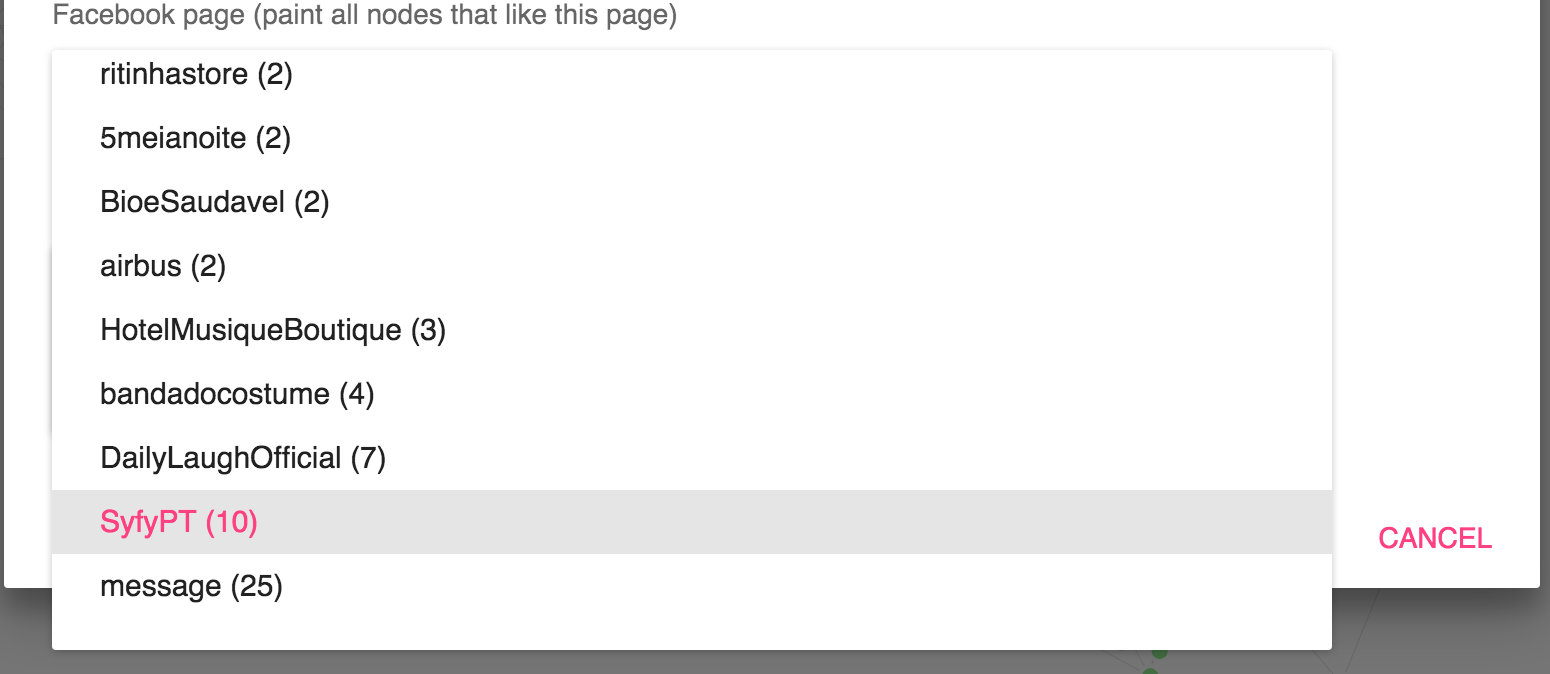
\includegraphics[width=1.2\textwidth]{img/socii/socii_9.png}
\end{center}
\caption{\label{img:socii_10} Community detection for facebook page likes. \textit{SyfyPT} is a Facebook page.}
\end{figure}

As we can see in Figure \ref{img:socii_10} one may select among a variety of Facebook pages, note that after each page id we have the number of Facebook likes within the all network.

\begin{figure}[h!]
\begin{center}
  \hspace*{-0.8in}
  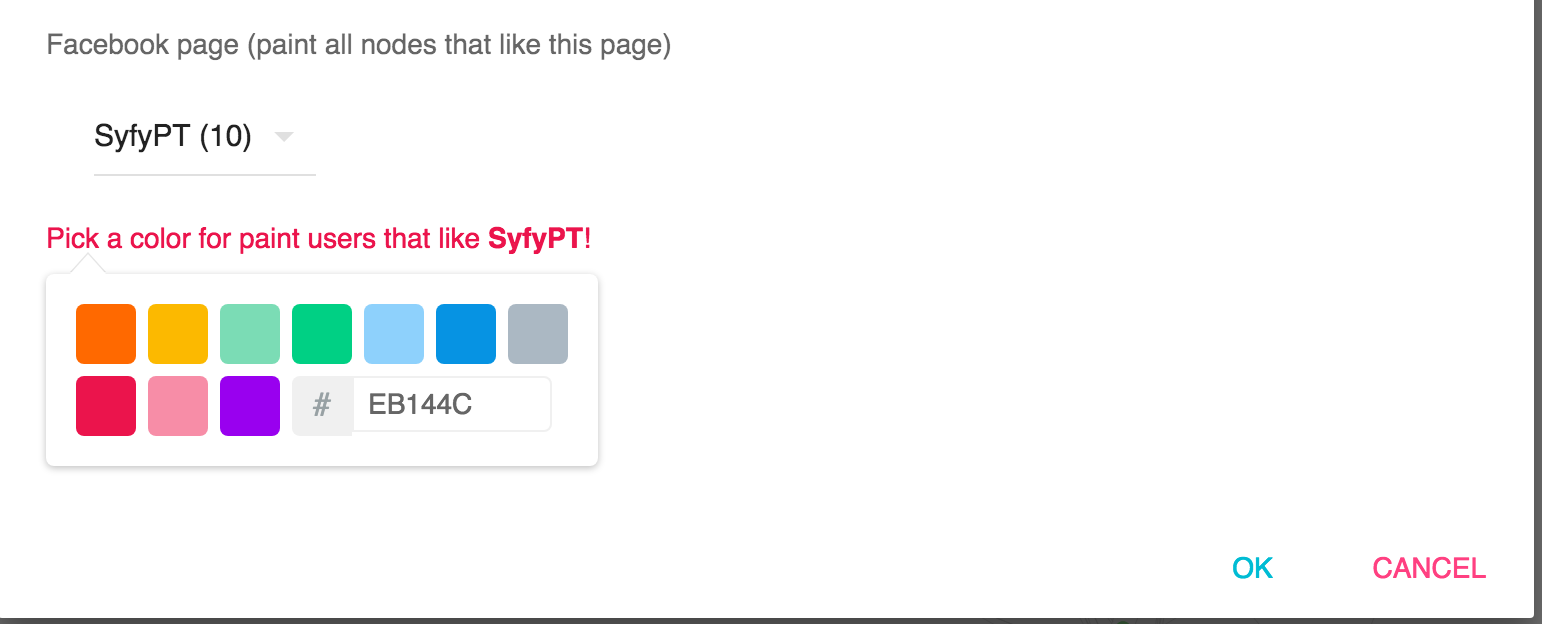
\includegraphics[width=1.2\textwidth]{img/socii/socii_10.png}
\end{center}
\caption{\label{img:socii_11} Community detection for facebook page likes. Picking a color.}
\end{figure}

\indent After choosing the page from the dropdown in Figure \ref{img:socii_10} we may see that the user is prompted with a color palette and a color input field. The user may either pick an already available color, or it may choose instead to insert the color code directly in the input field.

\indent Next after the user performs the previous two steps and clicks in the \textbf{"OK"} button the nodes in the network are coloring accordingly, a \textcolor{red}{red} label (\textit{chip} visual element) appears on the top left corner of the network visualization area and the so that the user knows what the color represents. In the specific case of Figure \ref{img:socii_11} all the \textcolor{red}{red} nodes \textit{like} the \textbf{SyfyPT} Facebook page \footnote{Aside note: if one wants actually to access the Facebook page one just needs to navigate into \url{https://facebook.com/SyfyPT}, if we have a open Facebook session the page will open in our browser}.

%% \subsubsection*{Community by LinkedIn skills}

\clearpage

%% ---------------------------------------------- Case Study
\section{Case Study}
Now that we exaustivelly presented all Socii features, we will know present how can we use them and derive some conclusions from network observation and analysis.\\
\indent As we mentioned Socii uses generators to build a network for a given \gls{osn} with a specific required number of nodes. In this section we present a real case study with real data in order to prove the accuracy of conclusions that Socii provides in a real context. For this case study we will use a real account and extract information from Facebook using the respective web crawler module that was developed initially as a back-end requirements to allow extraction on the fly, but not that being possible by the mentioned reasons, we use it as mean to obtain a real data set that we inject in Socii and associate to a whitelisted Socii account that besides being able of generating \glspl{osn} networks as normal users, the whitelisted users will also have available an option to consult a predefined network that is built on the fly with already stored data (the case study data).

\subsubsection{Detecting active and influent Facebook users}
Image. How to trace important users in the network that are very active.
\begin{enumerate}
    \item Stop the network.
    \item Rearrange the network to better suite visualization needs for that one may use features such as network drag and drop, network zooming, and node drag and drop.
    \item Turn on node discovery (optionally turn on node labels).
    \item Search for central nodes with degree above the average node degree within the network
    \item Turn on node comparison.
    \item Compare the previously group of central nodes and choose the one that has the highest eigenvector centrality
    and betweenness centrality and highest average Facebook reactions per post.
    \item If the previously steps lead to a specific node we may conclude that we found the most active and influent user in our network. Active because it simply posts with a certain frequency and influent because of the \textbf{interception of \gls{sna} metrics that lead us to a specific individual and \gls{osn} Facebook specific data that tells us that this particular user is socially (online) active and has a significat impact on other users since they react to its posts}.
    %SOLUTION: Maria Granja, Cluster de Amarante (com ligações a Braga), substituír nomes concretos por letras!!! Todos os dados dever ser incógnitas
\end{enumerate}

Following the previous \textit{"script"} one may find using Socii the most influent and active Facebook user. Using node metrics such as \textbf{degree centrality} and \textbf{average degree centrality} we can easaly capture users that have many connections, also features like network discovery are thought to help users understands nodes underlying connections. \glspl{osn} specific metrics (e.g. \textbf{average reactions per posts} may indicate us what users are well established in terms of Facebook activity).

\subsubsection{Marketing with community detection (Facebook)}
A real example within the case study. Study community preferences.

\begin{enumerate}
    \item Stop the network.
    \item Rearrange the network to better suite visualization needs for that one may use features such as network drag and drop, network zooming, and node drag and drop.
    \item Turn on node discovery (optionally turn on node labels);
    \item Open community detection dialog and find the marketing target (this is a Facebook page, it may be a brand a tv channel etc.);
    \item Color the nodes that likes this certain marketing target;
    \item Within the colored nodes find the most active and influent (we explained how to obtain this nodes in the previous section);
\end{enumerate}

By performing the following steps we may then plan a market strategy upon a certain group of individuals that may be implemented in all sorts of forms such as:
\begin{itemize}
    \item Send newsletters directly to the target users;
    \item Try and reach the target users personally;
    \item Save data and cross results with another networks in order to launch public campaign.
\end{itemize}

%% \subsubsection{HR Discovery (LinkedIn)} ONLY IF TIME!!!!!!!!!!
